%% LyX 2.3.5.2 created this file.  For more info, see http://www.lyx.org/.
%% Do not edit unless you really know what you are doing.
\documentclass[english,aspectratio = 169,  serif, mathserif, professionalfont]{beamer}
\PassOptionsToPackage{natbib=true}{biblatex}
\usepackage[T1]{fontenc}
\usepackage[latin9]{inputenc}
\usepackage{booktabs}
\usepackage{bm}
\usepackage{amstext}
\usepackage{amsthm}
\usepackage{graphicx}

\makeatletter

%%%%%%%%%%%%%%%%%%%%%%%%%%%%%% LyX specific LaTeX commands.
%% Because html converters don't know tabularnewline
\providecommand{\tabularnewline}{\\}
%% A simple dot to overcome graphicx limitations
\newcommand{\lyxdot}{.}


%%%%%%%%%%%%%%%%%%%%%%%%%%%%%% Textclass specific LaTeX commands.
% this default might be overridden by plain title style
\newcommand\makebeamertitle{\frame{\maketitle}}%
% (ERT) argument for the TOC
\AtBeginDocument{%
  \let\origtableofcontents=\tableofcontents
  \def\tableofcontents{\@ifnextchar[{\origtableofcontents}{\gobbletableofcontents}}
  \def\gobbletableofcontents#1{\origtableofcontents}
}
\theoremstyle{plain}
\newtheorem{thm}{\protect\theoremname}
\theoremstyle{plain}
\newtheorem{prop}[thm]{\protect\propositionname}
\theoremstyle{definition}
\newtheorem*{defn*}{\protect\definitionname}

%%%%%%%%%%%%%%%%%%%%%%%%%%%%%% User specified LaTeX commands.
%\usetheme{metropolis}
%\usetheme{Darmstadt}
\usetheme{default}
\setbeamertemplate{navigation symbols}{}

\usepackage[bottom]{footmisc}
\usepackage{placeins}
%\usepackage[adobe-utopia]{mathdesign}
\usepackage{pifont}
%\usepackage{kerkis}
%\usepackage{pxfonts}
\usepackage[default]{lato}
%\usepackage{mathpazo}
\usepackage{eulervm}



\usepackage{dcolumn}
\usepackage{bbm}
\newcolumntype{d}[0]{D{.}{.}{5}}

\usepackage{changepage}

\addtobeamertemplate{frametitle}{}{\vspace{-0.2 cm}}

\setbeamertemplate{frametitle} 
{ 
	\begin{centering} 
		\LARGE
		\insertframetitle
		\par 
	\end{centering} 
} 

\setbeamerfont{title}{size = \LARGE}





%COLORS
\definecolor{chamois}{RGB}{254,254,245}
\definecolor{oldchamois}{RGB}{255,255,240}
\definecolor{darkbrown}{RGB}{124,79,0}
\definecolor{UniBlue}{RGB}{65,55,203}
\definecolor{bordeaux}{RGB}{201,18,18}
\definecolor{redd}{RGB}{245,29,29}


\definecolor{hellgelb}{rgb}{1,1,0.8}
\definecolor{colKeys}{rgb}{0,0,1}
\definecolor{colIdentifier}{rgb}{0,0,0}
\definecolor{colComments}{rgb}{1,0,0}
\definecolor{colString}{rgb}{0,0.5,0}
\definecolor{textcolour}{rgb}{0.37,0.34,0.27}

\definecolor{ITgreen}{rgb}{0,204/256,0}

\iffalse
%LIN AT THE TOP
\usepackage{tikz}
\newcommand{\topline}{%
	\tikz[remember picture,overlay] {%
		\draw[bordeaux,thick] ([yshift=-1.4cm]current page.north west)-- ([yshift=-1.4cm,xshift=\paperwidth]current page.north west);}}

\addtobeamertemplate{frametitle}{
}{\topline%
}
\fi

%ITEMIZE SEP
\setlength{\itemsep}{10mm}
%BACKGROUND AND ITEMIZE
%\setbeamercolor{background canvas}{bg=chamois}
\setbeamercolor{itemize item}{fg=bordeaux}
%\setbeamertemplate{itemize item}{\maltese}
\setbeamercolor{itemize subitem}{fg=bordeaux}
\setbeamertemplate{itemize subitem}{$\diamondsuit$}

%ELEMENT COLORS
\setbeamercolor{title}{fg=UniBlue}
\setbeamercolor{frametitle}{fg=UniBlue}
\setbeamercolor{structure}{fg=textcolour}

%COLORS FIRST PAGE
\setbeamercolor{author}{fg=darkbrown}
\setbeamercolor{date}{fg=darkbrown!60}
\setbeamercolor{institute}{fg=darkbrown}

%BLOCK SPECS
\setbeamercolor{block title}{bg=UniBlue!30,fg=white}
\setbeamercolor{block body}{bg=UniBlue!10,fg=black}
%\addtobeamertemplate{block begin}{%
%	\centering
%	\setlength{\textwidth}{1\textwidth}%
%}{}

%\setbeamercolor{block title alerted}{bg=yellow!60,fg=red}
%\setbeamercolor{block body alerted}{bg=hellgelb!80,fg=UniBlue}


\setbeamercolor{alert}{fg=redd}
\renewcommand<>{\alert}[1]{%
	{\usebeamercolor[fg]{alert}\only#2{}#1}%
}

\newcommand{\blue}{\color{blue}}






\usepackage{tabularx}
\usepackage{booktabs}
\usepackage{epstopdf}
\usepackage{graphicx}



\newcolumntype{C}[1]{>{\centering\let\newline\\\arraybackslash\hspace{0pt}}m{#1}}
\newcolumntype{L}[1]{>{\flushleft\let\newline\\\arraybackslash\hspace{0pt}}m{#1}}
\newcolumntype{P}{>{\centering\arraybackslash}m{3cm}}
\renewcommand{\baselinestretch}{1.3} 
\usepackage{lscape}

%%% TIKZ %%%%
\usepackage{tikz}
\usetikzlibrary{positioning}
\usetikzlibrary{snakes}
\usetikzlibrary{calc}
\usetikzlibrary{arrows}
\usetikzlibrary{decorations.markings}
\usetikzlibrary{shapes.misc}
\usetikzlibrary{matrix,shapes,arrows,fit,tikzmark}
\usepackage{pgfplots}



\usepackage{dcolumn}
\usepackage{bbm}
\newcolumntype{d}[0]{D{.}{.}{5}}
\newcolumntype{C}[1]{>{\centering\let\newline\\\arraybackslash\hspace{0pt}}m{#1}}
\newcolumntype{L}[1]{>{\flushleft\let\newline\\\arraybackslash\hspace{0pt}}m{#1}}
\newcolumntype{P}{>{\centering\arraybackslash}m{3cm}}
\renewcommand{\baselinestretch}{1.3} 

\newcolumntype{H}{>{\setbox0=\hbox\bgroup}c<{\egroup}@{}}

%\usepackage{animate}

\makeatother

\usepackage{babel}
\usepackage[style=authoryear,backend=bibtex]{biblatex}
\providecommand{\definitionname}{Definition}
\providecommand{\propositionname}{Proposition}
\providecommand{\theoremname}{Theorem}

\begin{document}
\title{\thispagestyle{empty}Competing for Inventors: Market Concentration
and the Misallocation of Innovative Talent}
\author{Andrea Manera}
\date{October 5, 2021}

\makebeamertitle
%
\tikzset{            every picture/.style={remember picture,baseline},         every node/.style={anchor=base,align=center,outer sep=1.5pt},         every path/.style={thick}} 
\newcommand\marktopleft[1]{% 
   \tikz[overlay,remember picture]          \node (marker-#1-a) at (-.3em,.3em) {};% 
}
\newcommand\markbottomright[2]{%   
 \tikz[overlay,remember picture]          \node (marker-#1-b) at (0em,0em) {};%  
}
\tikzstyle{every picture}+=[remember picture] 
\tikzstyle{mybox} =[draw=black, very thick, rectangle, inner sep=10pt, inner ysep=20pt] 
\tikzstyle{fancytitle} =[draw=black,fill=red, text=white] 
\pgfplotsset{compat=1.9}
\pgfplotsset{every axis/.append style={            label style={font=\Large},                     tick label style={font=\Large}                       }}
%%%% END TIKZ STUFF

\section{Introduction}
\begin{frame}{Motivation}

\noindent \begin{columns}[T]
\begin{column}{.5\textwidth} 
\onslide<1-4>\begin{itemize}   
\item<1-> TFP growth has slowed down\\
\vspace{-.8em}
{\tiny{Fernald et al. (2014), Gordon (2016), Akcigit and Ates (2021)}}
\item<2-> R\&D productivity has fallen \\
\vspace{-.8em}
{\tiny{Bloom et al. (2020), Acemoglu et al. (2018, 2021)}}
\item<3-> Inventors have skills broader than product markets, high mobility\\
\vspace{-.8em}
{\tiny{Akcigit et al. (2016), Azoulay et al. (2017), Moretti et al. (2017)}}
\end{itemize} 
\end{column}% 
\hspace{-.2em}
\begin{column}{.5\textwidth}
\onslide<1-4>\only<1>{\resizebox{\textwidth}{!}{ 
\includegraphics{graphs/Akcigit_and_Ates_TFP_slowed.png}
}\\\vspace{-.8em}
{\centering\tiny{Source: Akcigit and Ates (2021)}}
}   
\onslide<1-4>\only<2-4>{\resizebox{\textwidth}{!}{ 
\includegraphics{graphs/Bloom_et_al.png}
}\\\vspace{-.8em}
{\centering\tiny{Source: Bloom et al. (2020)}}
}   
\end{column}% 
\end{columns}
\begin{center}
\bigskip{}
\textcolor{red}{\Large{}\onslide<4>{Are inventors and their skills  misallocated?}}{\Large\par}
\par\end{center}

\end{frame}

\begin{frame}{This Paper}
\begin{itemize}
\item \onslide<1->Inventors have become increasingly misallocated in the
last 20 years
\begin{itemize}
\item \onslide<2->employed by incumbents in less competitive sectors
\item \onslide<3->deployed to non-productive, defensive, R\&D projects
(``patent walls'')
\end{itemize}
\item \onslide<4->Mechanism:
\begin{itemize}
\item \onslide<5->Dominant firms engage in both productive and defensive
R\&D activities{\tiny{}}\\
{\tiny{}Hall and Helmers (2015), Abrams et al. (2018), Akcigit and
Kerr (2018), Jo (2019), Argente et al. (2021) }{\tiny\par}
\item \onslide<6->Defensive R\&D more attractive when profits to protect
are bigger\\
{\tiny{}Arrow's (1962) replacement effect}{\tiny\par}
\item \onslide<7->Concentration and profits have increased significantly
in the US\\
{\tiny{}Autor et al. (2020), Gutierrez and Philippon (2017, 2018),
Grullon et al. (2019), Barkai (2020), De Loecker et al. (2020)}{\tiny\par}
\item \onslide<8->Concentrating sectors attracted more inventors, pushing
growth below potential
\end{itemize}
\item \onslide<9->Misallocation can explain 7.5-22.5\% of fall in annual
growth (-.15pp to -.45pp)
\end{itemize}
\end{frame}
%
\begin{frame}{Roadmap}

\begin{itemize}
\item \onslide<1->Data construction
\begin{itemize}
\item \onslide<2->{Group sectors that compete for similar inventors}%\vspace{-2em}
\end{itemize}
\item \onslide<4-> Empirical analysis
\begin{itemize}
\item \onslide<5->{Sectors with growing concentration increased their share or inventors} 
\item \onslide<6->{Fall in inventors' productivity in concentrating sectors}%\vspace{-2em}
\end{itemize}
\item \onslide<7-> Model
\begin{itemize}
\item \onslide<8->{Schumpeterian model with defensive innovation} %\vspace{-.8em}
\end{itemize}
\item \onslide<9->{Calibration and Policy}
\begin{itemize}
\item \onslide<10->{Subsidize entrants in concentrated sectors}
\item \onslide<11->{Cost-neutral policy raises annual growth by .28pp}
\end{itemize}
\end{itemize}
\end{frame}
%

\section{Data Construction}

\begin{frame}{}

\vspace{2em}
\begin{center}
{\color{UniBlue} \Huge Data Construction}
\end{center}
\end{frame}
%
\begin{frame}{Empirical Analysis Objectives}
\begin{itemize}
\item Identify ``knowledge markets'': labor markets for inventors with
same skills
\begin{itemize}
\item Build a network of flows of inventors across sectors
\item Identify sets of product markets that hire the same type of inventors
\end{itemize}
\end{itemize}
\vspace{2em}
\begin{itemize}
\item \emph{Within knowledge markets: }
\begin{itemize}
\item Analyze how concentration and product markets' share of inventors
are related
\item Evaluate effects of increased concentration on R\&D productivity
\end{itemize}
\end{itemize}
\end{frame}
%
\begin{frame}{Data Sources}
\begin{itemize}
\item USPTO (patent-year) and Goldschlag et al. (2016): 
\begin{itemize}
\item patent citation and disambiguated inventor id's, 1975-present;
\item Cooperative Patent Classification (CPC) 
\item patent classification by NAICS of application (1978-2016)
\end{itemize}
\end{itemize}
\vspace{1em}
\begin{itemize}
\item Economic Census and Keil (2017) (5-year-NAICS)
\begin{itemize}
\item NAICS 4-digit concentration measure: HHI and HHI lower bound
\item Output per worker growth
\end{itemize}
\end{itemize}
\vspace{1em}
\begin{itemize}
\item NBER-CES:
\begin{itemize}
\item Constructed Lerner Index 
\end{itemize}
\end{itemize}
\end{frame}
%
\begin{frame}{``Knowledge Markets''}
\begin{itemize}
\item \emph{Ideally}: 
\begin{itemize}
\item set of product markets with same \emph{required knowledge }innovate
\end{itemize}
\end{itemize}
\vspace{2em}
\begin{itemize}
\item \emph{In practice:} 
\begin{itemize}
\item NAICS 4-digit sectors connected by flows of inventors 
\item Identify flows from patents with disambiguated inventors
\item Group NAICS that have strongest connections
\end{itemize}
\end{itemize}
\end{frame}
%
\begin{frame}{Building a Knowledge Market}
\begin{center}
\begin{figure}
\includegraphics[width=1\textwidth]{graphs/Kmarkets/Kmarkets\lyxdot 001}
\end{figure}
\par\end{center}

\end{frame}
%
\begin{frame}{Building a Knowledge Market}
\begin{center}
\begin{figure}
\includegraphics[width=1\textwidth]{graphs/Kmarkets/Kmarkets\lyxdot 002}
\end{figure}
\par\end{center}

\end{frame}
%
\begin{frame}{Building a Knowledge Market}
\begin{center}
\begin{figure}
\includegraphics[width=1\textwidth]{graphs/Kmarkets/Kmarkets\lyxdot 003}
\end{figure}
\par\end{center}

\end{frame}
%
\begin{frame}{Building a Knowledge Market}
\begin{center}
\begin{figure}
\includegraphics[width=1\textwidth]{graphs/Kmarkets/Kmarkets\lyxdot 004}
\end{figure}
\par\end{center}

\end{frame}
%
\begin{frame}{Building a Knowledge Market}
\begin{center}
\begin{figure}
\includegraphics[width=1\textwidth]{graphs/Kmarkets/Kmarkets\lyxdot 005}
\end{figure}
\par\end{center}

\end{frame}
%
\begin{frame}{Building a Knowledge Market}
\begin{center}
\begin{figure}
\includegraphics[width=1\textwidth]{graphs/Kmarkets/Kmarkets\lyxdot 006}
\end{figure}
\par\end{center}

\end{frame}
%
\begin{frame}{Constructing Inventor Flows}
 

\begin{table}
\begin{tabular}{|c|c|c|c|}
\hline 
Patent ID & Inventor ID & Goldschlag et al. (2016) NAICS & Year\tabularnewline
\hline 
\marktopleft{a1}US00001 & 00001-1 & 1111 & 1980\tabularnewline
US00001 & 00001-1 & 1112 & 1980\markbottomright{a1}{red}\tabularnewline
US00001 & 00001-2 & 1111 & 1980\tabularnewline
US00001 & 00001-2 & 1112 & 1980\tabularnewline
US00002 & 00001-1 & 3111 & 1981\tabularnewline
\hline 
\end{tabular}
\end{table}
\uncover<2->{\tikz[overlay,remember picture,inner sep=1pt] \node[draw=red,rounded corners,fit=(marker-a1-a.north west) (marker-a1-b.south east)] {};}
\end{frame}
%
\begin{frame}{Constructing Inventor Flows}

\begin{table}
\scalebox{.9}{%
\begin{tabular}{|c|c|c|c|}
\hline 
Patent ID & Inventor ID & Goldschlag et al. (2016) NAICS & Year\tabularnewline
\hline 
US00001 & 00001-1 & 1111 & 1980\tabularnewline
US00001 & 00001-1 & 1112 & 1980\tabularnewline
US00001 & 00001-2 & 1111 & 1980\tabularnewline
US00001 & 00001-2 & 1112 & 1980\tabularnewline
US00002 & 00001-1 & 3111 & 1981\tabularnewline
\hline 
\end{tabular}}
\end{table}

\begin{center}$\Downarrow \qquad \Downarrow \qquad \Downarrow $\end{center}

\begin{table}
\scalebox{.9}{%
\begin{tabular}{|c|c|c|c|}
\hline 
NAICS 1 & NAICS 2 & Year & Total Flows\tabularnewline
\hline 
1111 & 1112 & 1980 & 2\tabularnewline
\hline 
1112 & 3111 & 1981 & 1\tabularnewline
\hline 
\end{tabular}}
\end{table}

\end{frame}
%
\begin{frame}{Weighting Flows: ``Effective Inventors''}

\only<1>{
\begin{itemize}
\item Flows shall adjust for productivity of inventors who move
\end{itemize}
}\only<2->{
\begin{itemize}
\item \emph{Effective inventors:} 
\only<2->{\begin{itemize}
\item "Productivity-adjusted" inventor. Fixed effect  in regression:
\[\#Patents_{cfit}=\alpha_{i}+\alpha_{cft}+\varepsilon_{cfit}\]
\only<3->{\item $\alpha_{cft}$: CPC class 1-digit, $c$, by firm (assignee), $f$, by year, $t$, fixed effect}
\only<4>{\item Results robust to using raw number of inventors}
\end{itemize}}
\end{itemize}
}
\begin{itemize}
\item \emph{\onslide<6-> Effective inventor flow from sector 1 to 2:}
\begin{align*}
flow_{1\rightarrow2,t} & =\sum_{i}\#\left\{ \text{\ensuremath{i's\ transitions\ 1\rightarrow2\text{ \ensuremath{in} }t}}\right\} \cdot\alpha_{i}
\end{align*}
\end{itemize}
\end{frame}
%
\begin{frame}{Detecting Knowledge Markets}
\begin{itemize}
\item Total undirected flows:
\[
flow_{12}=\sum_{t}\left(flow_{1\rightarrow2,t}+flow_{2\rightarrow1,t}\right)
\]
used as network weights \hyperlink{appendix: Weights}{\beamergotobutton{Normalization}}\label{button: BackToFlows}
\item Maximize modularity of flow network over:
\begin{itemize}
\item Number of \emph{non-overlapping} communities $N$
\item Assignment of nodes to the $N$ communities
\end{itemize}
\item Density of links \emph{within }communities versus \emph{between} \hyperlink{appendix: Louvain}{\beamergotobutton{Formula and Algorithm}}\label{button: BackToComm}
\item Result: 10 non-singleton sets of NAICS 4-digit that share inventors
\end{itemize}
\end{frame}
%
\begin{frame}{Visualization at 3-digit NAICS}
\begin{center}
\begin{figure}
\includegraphics[height=0.9\paperheight]{graphs/Community_3d}
\end{figure}
\par\end{center}

\end{frame}
%
\begin{frame}{Features of Flows and Knowledge Markets}

\begin{columns}[T]
\begin{column}{.5\textwidth} 
\onslide<1-4>\vspace{2em}\begin{itemize}   
\item<1-> Iventor flows between many different product markets!
\item<2-> Orange: "Mining, Heavy Industry" \\
\vspace{-.8em}
{\tiny{Petroleum and Coal Products, Chemical, Machinery Manufacturing}}
\item<3-> Green: "Food and Agriculture" \\
\vspace{-.8em}
{\tiny{Crop Production, Food Manufacturing, Beverage and Tobacco}}
\item<4-> Yellow: "Communications, Electronics" \\
\vspace{-.8em}
{\tiny{Computer Products, Telecommunications, Data Processing}}
\end{itemize} 
\end{column}% 
\hspace{-1em}
\begin{column}{.6\textwidth}
\vspace{-1.3em}
\resizebox{\textwidth}{!}{ 
\includegraphics{graphs/Community_3d.png}
}
\end{column}% 
\end{columns}
\end{frame}
%

\section{Empirical Analysis}
\begin{frame}{}

\vspace{2em}
\begin{center}
{\color{UniBlue} \Huge Empirical Analysis}
\end{center}
\end{frame}
%

\begin{frame}{Variable Definition}

\begin{itemize}
\item Market concentration: $HHI$
\begin{itemize}
\item Economic Census does not compute $HHI$ for all sectors
\item But always reports top 4, 8, 20, 50 firms' share
\item Use $\underline{HHI}$: lower bound of HHI computed from top shares
(Keil, 2017) \label{button: BackToVariables}\hyperlink{appendix: HHILB}{\beamergotobutton{Expression}}
\end{itemize}
\item Sector $p$'s share of effective inventors in knowledge market, $k$:
\[
Inventor\ Share_{p,t}\equiv\frac{\sum_{p(i,t)=p}\alpha_{i}}{\sum_{k(i,t)=k}\alpha_{i}},
\]

\begin{itemize}
\item $\alpha_{i}$ are ``effective inventors'', or raw number of inventors
\vspace{5pt}
\item Averaged for 5 years \emph{starting }in census years {\tiny{}(same
results with symmetric window)}{\tiny\par}
\end{itemize}
\item Size of sectors or firms: real sales, real sales per company (Economic
Census)
\end{itemize}
\end{frame}
%
\begin{frame}{Specification}
\begin{itemize}
\item Long-difference 2012-1997 at NAICS 4-digit sector, $p$:
\[
\Delta Share{}_{p,\ 2012-1997}=f_{k}\mathbf{1}\left\{ p\in k\right\} \ +\ \beta\Delta HHI_{p,\ 2012-1997}\ +\ \gamma\Delta Size_{p,\ 2012-1997}\ +\ \varepsilon_{p},
\]
\item $f_{k}\mathbf{1}\left\{ p\in k\right\} $: sector $p$ belongs to
knowledge market $k$
\item $\Delta\text{HHI}_{p}:$ change in concentration
\item $\Delta Size_{p,\ 2012-1997}:$ log-real sales of sector, per firm
\item Weighted by sales, robust standard errors
\end{itemize}
\end{frame}
%
\begin{frame}{Main Specification Results \hyperlink{appendix: NoControls}{\beamergotobutton{No Controls}}\hyperlink{appendix: HHICensus}{\beamergotobutton{Census HHI}}\hyperlink{appendix: OutliersMain}{\beamergotobutton{Trim Outliers}}\hyperlink{appendix: NInv}{\beamergotobutton{Raw Inventors}}}
\label{button: BackToMainSpec}

\begin{table}
\begin{centering}
\input{tab/Dk4_sh_inv_hhi_inv_fe1SH.tex}\\
\par\end{centering}
\centering{}{\tiny{}Robust standard errors in parentheses, $+\ p<0.1,^{*}\ p<0.05,^{**}\ p<.01,^{***}\ p<.001$}{\tiny\par}
\end{table}

\end{frame}
%
\begin{frame}{Causality}

Threats to causal interpretation:
\begin{itemize}
\item Inventors move towards expanding sectors/firms 
\begin{itemize}
\item Control for change in sales
\item Control for change in sales per company
\end{itemize}
\item Reverse causality: increase in inventors drives higher concentration 
\begin{itemize}
\item Inventors' share computed on 5 years \emph{starting }in Economic Census
year
\item IV analysis using Mercatus regulation data \hyperlink{appendix: IV}{\beamergotobutton{Details}}\label{button: BackToCausality}
\end{itemize}
\end{itemize}
\end{frame}
%

\begin{frame}{Robustness to Individual Firm Size \hyperlink{appendix: OutliersSize}{\beamergotobutton{Robustness to Outliers}}\label{button: BackToMainSpec-2}}

\begin{table}
\begin{centering}
\input{tab/Dk4_sh_inv_hhi_pc_inv_fe1SH.tex}\\
\par\end{centering}
\centering{}{\tiny{}Robust standard errors in parentheses, $+\ p<0.1,^{*}\ p<0.05,^{**}\ p<.01,^{***}\ p<.001$}{\tiny\par}
\end{table}

\end{frame}
%
\begin{frame}{What Happens\emph{ }within Product Markets?\textcolor{blue}{\LARGE{} }}

\label{button: BackToWithinKMKT}An increase in inventor shares:
\begin{itemize}
\item Significantly increases
\begin{itemize}
\item Top 10\% firms' inventor shares, Top 10\%/Bottom 50\% ratio \hyperlink{appendix: WithinDist}{\beamergotobutton{Table}}
\item Self-citations \hyperlink{appendix: SelfCite}{\beamergotobutton{Table}}
\end{itemize}
\item Significantly decreases
\begin{itemize}
\item Inventors' productivity (next slide)
\item Patents' forward citations \hyperlink{appendix: FWDCite}{\beamergotobutton{Table}}
\end{itemize}
\end{itemize}
\end{frame}
%
\begin{frame}{Fall in Inventors' Productivity \hyperlink{appendix: InvProdFull}{\beamergotobutton{Robustness to Outliers}}}

\label{button: BackToInvProd}
\begin{figure}
\begin{centering}
{
\def\sym#1{\ifmmode^{#1}\else\(^{#1}\)\fi}
\begin{tabular}{l*{2}{c}HH}
\hline\hline
                    &$\Delta$ Growth/Inventor (pp)   &               &               &               \\
                    &\multicolumn{1}{c}{(1)}   &\multicolumn{1}{c}{(2)}   &\multicolumn{1}{H}{(3)}   &\multicolumn{1}{H}{(4)}   \\
\hline
$\Delta \underline{HHI}$  &      -0.332** &      -0.292*  &      -0.332** &      -0.290*  \\
                    &     (0.113)   &     (0.123)   &     (0.114)   &     (0.126)   \\
$\Delta \log$ Sales  &               &      -0.052*  &               &      -0.053*  \\
                    &               &     (0.021)   &               &     (0.022)   \\
\hline
Knowledge Market FE&   \ding{51}   &   \ding{51}   &   \ding{51}   &   \ding{51}   \\
Sample              & Full Sample   & Full Sample   &Mahalanobis 5\%   &Mahalanobis 5\%   \\
Weight              &       Sales   &       Sales   &       Sales   &       Sales   \\
Observations        &         101   &         101   &          98   &          94   \\
\hline\hline
\end{tabular}
}
\\
\par\end{centering}
\centering{}{\tiny{}Robust standard errors in parentheses, $+\ p<0.1,^{*}\ p<0.05,^{**}\ p<.01,^{***}\ p<.001$}{\tiny\par}
\end{figure}

\end{frame}
%
\begin{frame}{Back-of-the-envelope Loss from Misallocation}

Implied loss from misallocation for the median sector with $\Delta$
Inventor Share $>0$:

{\large{}\begin{equation*}
\onslide<1->{\Delta g=\only<1>{\frac{\Delta\left(\frac{g}{Inventor}\right)}{\Delta\underline{HHI}}}%
\only<2-5>{\underset{\text{-.29}}{\underbrace{\frac{\Delta\left(\frac{g}{Inventor}\right)}{\Delta\underline{HHI}}}}}%
\only<6->{\underset{\in[-.54,-.05]}{\underbrace{\frac{\Delta\left(\frac{g}{Inventor}\right)}{\Delta\underline{HHI}}}}}%
\only<1-2>{\times\Delta\underline{HHI}}
\only<3->{\times\underset{.0019}{\underbrace{\Delta\underline{HHI}}}}
\only<1-3>{\times Inventors}
\only<4->{\times\underset{1421}{\underbrace{Inventors}}} 
\onslide<5->{\only<5>{=-0.78pp}\only<6->{\in [-1.45pp, -.13pp]}}
}
\end{equation*}
\onslide<7->{
\begin{itemize}
\item Compares to a median of $-2.73pp$
\onslide<8->{\item Misallocation would explain $28.6\%$ of this fall (4.8\% to 53\%)}
\onslide<9->{\item 23\% fall in output per worker growth for these sectors relative to 1997}
\onslide<10->{\item Similar results regressing of inventors' productivity on $\Delta$ Inventor Share} 
\end{itemize}
}}
\end{frame}
%
\begin{frame}{Recap of Key Results}
\begin{itemize}
\item Within knowledge markets:
\begin{itemize}
\item Sector that become more concentrated attract more inventors
\end{itemize}
\item Within product markets, increasing concentration:
\begin{itemize}
\item Lowers inventors' productivity (growth per inventor)
\item Increases share of inventors at top firms
\item Lowers forward citations
\end{itemize}
\end{itemize}
\end{frame}
%

\section{Theoretical Framework}
\begin{frame}{}

\vspace{2em}
\begin{center}
{\color{UniBlue} \Huge Model} 
\end{center}
\end{frame}
%
\begin{frame}{Model Objectives}
\begin{itemize}
\item Explain mechanism behind empirical facts
\item Schumpeterian model \emph{with defensive innovation} 
\begin{itemize}
\item Entrants give creative-destruction growth
\item Incumbents can engage in defensive innovation raising entrants' costs
\end{itemize}
\item Calibrate two sectors, one knowledge market model to evaluate policy:
\begin{itemize}
\item Optimal to subsidize entrants in concentrated sectors
\item Cost-neutral policy gives up to .155pp higher annual growth
\end{itemize}
\end{itemize}
\end{frame}
%
\begin{frame}{Single-Sector: Market Structure \hyperlink{appendix: ConcLerner}{\beamergotobutton{Concentration v. Markup}}}

\label{button: BackToSS} Consumption good is C-D of intermediates:
\[
Y_{t}=\int_{0}^{1}y_{t}(i)\mathrm{d}i
\]

Intermediate, $i$, produced with linear technology by either:
\begin{itemize}
\item Incumbent: unit cost $\frac{c_{t}(i)}{\phi},$ $\phi>1$; or
\item Entrants: unit cost $c_{t}(i)$
\end{itemize}
Bertrand competition, incumbent sets $p_{t}(i)=c_{t}(i)$, realizes
monopoly profits:
\[
\Pi_{t}=\left(\frac{\phi-1}{\phi}\right)c_{t}(i)y_{t}(i)=\left(\frac{\phi-1}{\phi}\right)Y_{t}.
\]

\end{frame}
%
\begin{frame}{Innovation}

Entrants and incumbents can invest in R\&D to obtain an innovation
reducing costs to:
\[
c_{t+\Delta t}=\frac{c_{t}}{\left(1+\eta\right)\phi},
\]
If innovation is \emph{implemented, }cost of all other firms drops
to:
\[
c_{t+\Delta t}=\frac{c_{t}}{\left(1+\eta\right)}
\]
Normalized incumbents' profits are constant:
\[
\pi_{t}\equiv\frac{\Pi_{t}}{Y_{t}}=\left(\frac{\phi-1}{\phi}\right)
\]

\end{frame}
%
\begin{frame}{Incumbents' R\&D}
\begin{itemize}
\item Incumbents' R\&D gives:
\begin{itemize}
\item a\emph{ patent wall} of size $\omega>1$ w.p. 1, which raises entrants'
costs,
\item an innovation w.p. $\lambda\in[0,1]$.
\end{itemize}
\item State of each market is the size of patent wall $\Omega\in\left\{ 1,\omega\right\} $
\item Incumbents choose an innovation intensity $x_{I}$ with costs:
\[
C\left(x_{I};w^{RD}\right)=\alpha_{I}\frac{x_{I}^{\gamma}}{\gamma}w^{RD},\ \gamma>1
\]
\item $\alpha_{I}\frac{x_{I}^{\gamma}}{\gamma}$ total incumbents' inventors
\item Fix $w^{RD}=1$ for now
\end{itemize}
\end{frame}
%
\begin{frame}{Incumbents' Values}

\begin{itemize}
\item Incumbents' normalized values $v=\frac{V\left(\Omega\right)}{Y}$
with constant output growth:
\begin{align*}
\rho v(1) & =\max_{x_{I}}\left(\frac{\phi-1}{\phi}\right)-\alpha_{I}\frac{x_{I}^{\gamma}}{\gamma}+x_{I}\left(v(\omega)-v(1)\right)-x_{e,1}\left(v(1)\right)\\
\rho v(\omega) & =\left(\frac{\phi-1}{\phi}\right)+\delta\left(v(1)-v(\omega)\right)-x_{e,\omega}\left(v(\omega)\right)
\end{align*}
\item $x_{e,1},x_{e,\omega}$: total research intensity of entrants 
\item $\delta$: depreciation of patent wall (patent protection)
\item Gain from innovation depends on the difference between $x_{e,\omega}$
and $x_{e,1}$
\end{itemize}
\end{frame}
%
\begin{frame}{Entrants}
\begin{itemize}
\item Successful entrants destroy any existing patent wall and get ``unprotected
value'' $v(1)$
\item Entrants are atomistic, mass determined in equilibrium
\item Crowding externalities in entrants' research (Abrams et al., 2018)
\item Linear cost $\zeta$$\times\Omega$:
\[
\max_{x_{e,\Omega,i}}x_{e,\Omega,i}v(1)-\zeta\Omega x_{e,\Omega,i}x_{e,\Omega}.
\]
\item Finite demand IFF:
\[
x_{e,\Omega}=\frac{v(1)}{\zeta\Omega}
\]
\item Total entrants' inventors sector with wall $\Omega$ given by $v(1)=\zeta\Omega x_{e,\Omega}$
\end{itemize}
\end{frame}
%
\begin{frame}{Growth and Inventors' Productivity \hyperlink{appendix: CGDef}{\beamergotobutton{Equilibrium Definition}}}

\label{button: BackToGrowth}Stationary distribution with constant
growth: \hyperlink{appendix: StatDist}{\beamergotobutton{Derivation}}
\[
\bm{\mu}=\left[\begin{matrix}\mu_{1} & \mu_{\omega} & \mu_{e,1} & \mu_{e,\omega}\end{matrix}\right]
\]
Growth is given by:
\[
g=\eta\left(x_{e,\omega}\mu_{e,\omega}+x_{e,1}\mu_{e,1}+\lambda x_{I}\mu_{1}\right)
\]
Inventors' productivity (growth per inventor):
\[
\frac{g}{L^{RD}}=\eta\frac{x_{e,\omega}\mu_{e,\omega}+x_{e,1}\mu_{e,1}+\lambda x_{I}\mu_{1}}{\zeta\left(\omega x_{e,\omega}\mu_{e,\omega}+x_{e,1}\mu_{e,1}\right)+\alpha_{I}\frac{x_{I}^{2}}{2}\mu_{1}}.
\]

\end{frame}
%
%
\begin{frame}{One-Sector Equilibrium Proposition }

\begin{prop}
\label{prop: partialEq-2}Consider the above model with a perfectly
elastic production and R\&D labor supply. Assume $\delta,\lambda=0,$
and 
\[
\sqrt{\frac{\phi-1}{\phi}}\left(\frac{\alpha_{I}-\zeta\omega\left(\omega-1\right)}{\alpha_{I}\zeta\omega}\right)>\rho.
\]
 An increase in the markup factor $m\equiv\frac{\phi-1}{\phi}$, increases
incumbents' and entrants' R\&D, growth, and the incumbents' share
of total R\&D labor, and decreases inventor productivity, $g/L^{RD}.$
\end{prop}

\begin{itemize}
\item Sufficient conditions, holds for wider range of parameters in simulations
\end{itemize}
\end{frame}
%
\begin{frame}{Single Sector Comparative Statics: Markup Increase}

\begin{columns}[T]
\begin{column}{.5\textwidth} 
\makebox[\linewidth][c]{ 
   \resizebox{\linewidth}{!}{
		% This file was created by matlab2tikz.
%
%The latest updates can be retrieved from
%  http://www.mathworks.com/matlabcentral/fileexchange/22022-matlab2tikz-matlab2tikz
%where you can also make suggestions and rate matlab2tikz.
%
\definecolor{mycolor1}{rgb}{0.00000,0.44700,0.74100}%
\definecolor{mycolor2}{rgb}{0.85000,0.32500,0.09800}%
%

\begin{tikzpicture}[every plot/.append style={line width=4pt}, ]
\tikzstyle{every node}=[font=\Large]

\only<1-3>{
\begin{axis}[%
width=\textwidth,
height=.8\textwidth,
at={(.1in,6in)},
scale only axis,
xmin=1.08,
xmax=1.98,
xlabel style={font=\color{white!15!black}\Large},
xlabel={Markup},
ymin=1,
ymax=6.68181818181818,
axis background/.style={fill=white},
title style={font=\bfseries\Large},
title={Profits},
%xticklabel shift={.5cm},
%yticklabel shift={.5cm}
]
\addplot [color=mycolor1, forget plot]
  table[row sep=crcr]{%
1.08	1\\
1.18	2.0593220338983\\
1.28	2.953125\\
1.38	3.71739130434782\\
1.48	4.37837837837838\\
1.58	4.95569620253164\\
1.68	5.46428571428571\\
1.78	5.91573033707865\\
1.88	6.31914893617021\\
1.98	6.68181818181818\\
};
\end{axis}
}


\only<4>{
\begin{axis}[%
width=\textwidth,
height=.8\textwidth,
at={(.1in,6in)},
scale only axis,
xmin=1.08,
xmax=1.98,
xlabel style={font=\color{white!15!black}\Large},
xlabel={Markup},
ymin=0.698336868435167,
ymax=1,
axis background/.style={fill=white},
title style={font=\bfseries\Large},
title={Inventor Productivity}
]
\addplot [color=mycolor1, forget plot]
  table[row sep=crcr]{%
1.08	1\\
1.18	0.899657487207735\\
1.28	0.849854954298308\\
1.38	0.818356595435947\\
1.48	0.796153368269253\\
1.58	0.779475419577032\\
1.68	0.766405201193097\\
1.78	0.755844174946435\\
1.88	0.747109891577814\\
1.98	0.739752568480054\\
};
\end{axis}
}
\end{tikzpicture}%
		}
	} 
\end{column}% 
\hspace{-.4em}
\begin{column}{.525\textwidth}
\only<2->{   
\makebox[\linewidth][c]{ 
   \resizebox{\linewidth}{!}{
		% This file was created by matlab2tikz.
%
%The latest updates can be retrieved from
%  http://www.mathworks.com/matlabcentral/fileexchange/22022-matlab2tikz-matlab2tikz
%where you can also make suggestions and rate matlab2tikz.
%
\definecolor{mycolor1}{rgb}{0.00000,0.44700,0.74100}%
\definecolor{mycolor2}{rgb}{0.85000,0.32500,0.09800}%
%


\begin{tikzpicture}[every plot/.append style={line width=4pt}, ]
 \tikzstyle{every node}=[font=\Large]


\begin{axis}[%
width=\textwidth,
height=.8\textwidth,
at={(.1in,6in)},
scale only axis,
area style,
stack plots=y,
xmin=1.13,
xmax=2.01,
xlabel style={font=\color{white!15!black}\Large},
xlabel={Markup},
ymin=0,
ymax=305.77273199311,
axis background/.style={fill=white},
title style={font=\bfseries\Large},
title={Inventors},
legend style={at={(0.5,-0.25)}, legend columns = -1, anchor=north, legend cell align=left, align=left, fill=none, draw=none}
]
\addplot[fill=mycolor1, draw=none] table[row sep=crcr]{%
1.13	70.0000551296365\\
1.14	72.3848037630461\\
1.15	74.6572719293103\\
1.16	76.8280536139858\\
1.17	78.9061701731101\\
1.18	80.8993836502963\\
1.19	82.8144335457369\\
1.2	84.6572188025262\\
1.21	86.4329398067949\\
1.22	88.1462106854136\\
1.23	89.801149192853\\
1.24	91.4014494477301\\
1.25	92.9504413760408\\
1.26	94.4511397315242\\
1.27	95.9062848554095\\
1.28	97.3183768256632\\
1.29	98.6897042688743\\
1.3	100.02236882737\\
1.31	101.318306060742\\
1.32	102.579303402209\\
1.33	103.807015665311\\
1.34	105.002978500201\\
1.35	106.168620123838\\
1.36	107.30527158962\\
1.37	108.414175814689\\
1.38	109.496495544953\\
1.39	110.55332040787\\
1.4	111.585673178931\\
1.41	112.594515367421\\
1.42	113.580752210138\\
1.43	114.545237148539\\
1.44	115.488775854403\\
1.45	116.412129858019\\
1.46	117.316019827254\\
1.47	118.201128537329\\
1.48	119.068103566462\\
1.49	119.917559748727\\
1.5	120.750081409537\\
1.51	121.566224408144\\
1.52	122.366518006472\\
1.53	123.151466582143\\
1.54	123.921551202173\\
1.55	124.677231070031\\
1.56	125.418944859527\\
1.57	126.147111945046\\
1.58	126.862133539038\\
1.59	127.564393744024\\
1.6	128.254260528154\\
1.61	128.932086629844\\
1.62	129.598210398965\\
1.63	130.252956578772\\
1.64	130.896637034347\\
1.65	131.529551432159\\
1.66	132.151987873658\\
1.67	132.764223488124\\
1.68	133.366524986523\\
1.69	133.959149180887\\
1.7	134.542343470445\\
1.71	135.116346297916\\
1.72	135.681387578325\\
1.73	136.237689101244\\
1.74	136.78546490998\\
1.75	137.324921657831\\
1.76	137.85625894452\\
1.77	138.379669632757\\
1.78	138.895340147217\\
1.79	139.403450757185\\
1.8	139.904175842958\\
1.81	140.397684148469\\
1.82	140.88413902003\\
1.83	141.363698632565\\
1.84	141.836516203576\\
1.85	142.302740196829\\
1.86	142.762514514828\\
1.87	143.21597868184\\
1.88	143.663268018079\\
1.89	144.10451380448\\
1.9	144.539843440154\\
1.91	144.969380591838\\
1.92	145.393245336337\\
1.93	145.811554295768\\
1.94	146.224420767282\\
1.95	146.631954845932\\
1.96	147.034263542287\\
1.97	147.431450894502\\
1.98	147.823618075757\\
1.99	148.210863496061\\
2	148.593282900343\\
2.01	148.970969461851\\
}
\closedcycle;
\addlegendentry{Entrants}
\only<3->{
\addplot[fill=mycolor2, draw=none] table[row sep=crcr]{%
1.13	29.9999448810842\\
1.14	32.3141239665027\\
1.15	34.6046135488823\\
1.16	36.8705995254392\\
1.17	39.1114842458398\\
1.18	41.3268435953698\\
1.19	43.5163937610695\\
1.2	45.6799651371986\\
1.21	47.8174815908121\\
1.22	49.9289438110575\\
1.23	52.0144158143589\\
1.24	54.0740139176259\\
1.25	56.1078976628475\\
1.26	58.1162623003677\\
1.27	60.0993325278174\\
1.28	62.0573572489438\\
1.29	63.9906051670595\\
1.3	65.8993610663018\\
1.31	67.7839226624017\\
1.32	69.6445979285435\\
1.33	71.4817028192093\\
1.34	73.2955593288746\\
1.35	75.086493833655\\
1.36	76.8548356732361\\
1.37	78.6009159375347\\
1.38	80.3250664281007\\
1.39	82.0276187691972\\
1.4	83.7089036477222\\
1.41	85.3692501641999\\
1.42	87.0089852794474\\
1.43	88.6284333439297\\
1.44	90.227915699244\\
1.45	91.8077503415917\\
1.46	93.3682516398394\\
1.47	94.9097301005647\\
1.48	96.4324921739811\\
1.49	97.9368400960669\\
1.5	99.423071761512\\
1.51	100.89148062438\\
1.52	102.34235562233\\
1.53	103.775981121393\\
1.54	105.192636879245\\
1.55	106.592598023829\\
1.56	107.976135046208\\
1.57	109.343513804868\\
1.58	110.694995540857\\
1.59	112.030836901371\\
1.6	113.351289971626\\
1.61	114.656602312921\\
1.62	115.947017006987\\
1.63	117.222772704742\\
1.64	118.484103679354\\
1.65	119.731239883109\\
1.66	120.964407006537\\
1.67	122.183826540652\\
1.68	123.389715840519\\
1.69	124.582288191065\\
1.7	125.761752873503\\
1.71	126.928315232869\\
1.72	128.082176746492\\
1.73	129.223535092151\\
1.74	130.35258421716\\
1.75	131.46951440677\\
1.76	132.574512353124\\
1.77	133.667761223258\\
1.78	134.749440726908\\
1.79	135.819727184053\\
1.8	136.878793591151\\
1.81	137.92680968731\\
1.82	138.96394201935\\
1.83	139.990354006176\\
1.84	141.006206001842\\
1.85	142.011655358469\\
1.86	143.006856487432\\
1.87	143.991960919839\\
1.88	144.967117366313\\
1.89	145.932471774967\\
1.9	146.888167389085\\
1.91	147.834344803382\\
1.92	148.771142019358\\
1.93	149.698694499161\\
1.94	150.61713521923\\
1.95	151.526594722058\\
1.96	152.427201167306\\
1.97	153.319080381693\\
1.98	154.202355908313\\
1.99	155.077149054038\\
2	155.943578936767\\
2.01	156.801762531259\\
}
\closedcycle;
\addlegendentry{Incumbents}
}
\end{axis}

\end{tikzpicture}%
		}
	}
}
\end{column}% 
\end{columns}

\end{frame}
%
\begin{frame}{Two-Sectors, Inventor Market Equilibrium}
\begin{itemize}
\item Two Cobb-Douglas sectors as above:
\[
Y=\left[\int_{0}^{1}y_{1,t}(i)\mathrm{d}i\right]^{\beta_{1}}\left[\int_{0}^{1}y_{2,t}(i)\mathrm{d}i\right]^{1-\beta_{1}}
\]
\item Researchers now earn $w^{RD},$ separate market from production
\item Inventors' market clearing:
\begin{align*}
L^{RD,s}\left(w^{RD}\right) & =\sum_{i=1,2}\left\lbrace \mu_{1,i}\left(w^{RD}\right)\alpha_{I}\frac{x_{I,i}^{2}\left(w^{RD}\right)}{2}+\right.\\
 & \left.+\mu_{\omega,i}\left(w^{RD}\right)\zeta_{i}\omega_{i}x_{e,\omega,i}\left(w^{RD}\right)+\mu_{1,e,i}\left(w^{RD}\right)\zeta_{i}x_{e,1,i}\left(w^{RD}\right)\right\rbrace 
\end{align*}
\item Normalize $L^{RD,s}=100.$ 
\end{itemize}
\end{frame}
%

\section{Calibration and Policy }
\begin{frame}{Calibration}
 

\begin{tabular}{L{3cm}C{2cm}C{1cm}L{1cm}C{3cm}}
\toprule  
Parameter Name & Symbol & \multicolumn{2}{c}{Value} & Source/Target \\ \midrule \midrule  
Discount rate & $\rho$ & .&04 & Annual real interest rate of $4\%$\\
Shares of Sectors' Value Added & $\beta$ & .&5 & Share of sales of sectors that saw an increase in HHI over total $\approx.5$\\
Average Sectors' Markup, Technology Gap & $\phi$ & 1&13 & Incumbent efficiency from Aghion et al. (2019)\\
Curvature of Innovation Function & $\gamma$ & \multicolumn{2}{c}{$1/.6$} & Lower bound of estimates in Kortum (1993)\\ 
Intensity of Patent Expiration & $\delta$ & .&05 & Uruguay Round Agreements Act (1994)\\
Share of Implemented Innovations & $\lambda$ & .&785 & Internal patent share of 21.5\% (Akcigit and Kerr, 2018)\\
Blocking Value of Patents & $\omega$ & 1.&469 & El. of Entry to patents from Hall and Helmers (2015)\\ \bottomrule 
\end{tabular} 
\begin{itemize}
\item Objective: study policy, provide \emph{lower bound of growth effects}
\item Match only R\&D statistics and Lerner Index gaps
\item Produces about $20\%$ of lower bound growth loss from empirics
\item Internal calibration for $\alpha_{I},\text{\ensuremath{\zeta},\ensuremath{\eta}},$
target incumbents' R\&D share, Business R\&D Share, avg. GDP growth
1997-2012\hyperlink{appendix: FullIntCal}{\beamergotobutton{Values}}
\item External calibration for the rest\hyperlink{appendix: FullExtCal}{\beamergotobutton{All Parameters}}\label{button: BackToCal}
\begin{itemize}
\item $\beta=.5$: sectors that saw an increase in Lerner Index ($\approx50\%$)
\item $\phi=1.13$ (Aghion et al., 2019)
\item $\omega=1.469$ (el. of entry to patents Hall and Helmers (2015))
\item $\lambda=.785$ ($21\%$ internal patents, Akcigit and Kerr (2018))
\item $\tau,s$: corp. tax $23\%$ and R\&D subsidy $19\%$ (Akcigit et
al.)
\end{itemize}
\end{itemize}
\end{frame}
%
\begin{frame}{CS: Increase in Sector 2 Markup \hyperlink{appendix: GraphSectors}{\beamergotobutton{Sector Aggregates}}\label{button: BackToCS2-1}}

\makebox[\textwidth][c]{ 
   \resizebox{.8\textwidth}{!}{  
		% This file was created by matlab2tikz.
%
%The latest updates can be retrieved from
%  http://www.mathworks.com/matlabcentral/fileexchange/22022-matlab2tikz-matlab2tikz
%where you can also make suggestions and rate matlab2tikz.
%
\definecolor{mycolor1}{rgb}{0.00000,0.44700,0.74100}%
\definecolor{mycolor2}{rgb}{0.85000,0.32500,0.09800}%
\definecolor{mycolor3}{rgb}{0.92900,0.69400,0.12500}%
\definecolor{mycolor4}{rgb}{0.49400,0.18400,0.55600}%
%


\begin{tikzpicture}[every plot/.append style={line width=.1pt}, ]
 \tikzstyle{every node}=[font=\LARGE]

\begin{axis}[%
width=1.6\textwidth,
height=.9\textwidth,
at={(.1in,6in)},
scale only axis,area style,
stack plots=y,
xmin=1,
xmax=2,
xlabel style={font=\color{white!15!black}\LARGE},
xlabel={Relative Markup},
ymin=0,
ymax=100.000000010722,
axis background/.style={fill=white},
title style={font=\bfseries\LARGE},
title={Inventors},
legend style={at={(0.5,-0.12)}, scale=.5, font=\LARGE, legend columns = -1, anchor=north, legend cell align=left, align=left, fill=none, draw=none}
]
\only<1>{
\addplot[fill=mycolor1, draw=mycolor1] table[row sep=crcr]{%
	1	35.000023681966\\
	1.1	27.8341246330096\\
	1.2	24.4115622110472\\
	1.3	22.3413645133138\\
	1.4	20.9360189051779\\
	1.5	19.912679610194\\
	1.6	19.1311494470074\\
	1.7	18.5132385976615\\
	1.8	18.0115980630876\\
	1.9	17.5957493561352\\
	2	17.2451237594452\\
}
\closedcycle;
\addlegendentry{Sector 1}

\addplot[fill=mycolor1, draw=mycolor1, forget plot] table[row sep=crcr]{%
	1	14.9999763240631\\
	1.1	9.003350310262\\
	1.2	6.70310647136026\\
	1.3	5.48552225210627\\
	1.4	4.73271616140255\\
	1.5	4.22173406059369\\
	1.6	3.85245693678996\\
	1.7	3.57326984412274\\
	1.8	3.35487742391974\\
	1.9	3.17942508524441\\
	2	3.03541548943501\\
}
\closedcycle;
}


\only<2->{
	\addplot[fill=mycolor1, draw=black] table[row sep=crcr]{%
	1	35.000023681966\\
	1.1	27.8341246330096\\
	1.2	24.4115622110472\\
	1.3	22.3413645133138\\
	1.4	20.9360189051779\\
	1.5	19.912679610194\\
	1.6	19.1311494470074\\
	1.7	18.5132385976615\\
	1.8	18.0115980630876\\
	1.9	17.5957493561352\\
	2	17.2451237594452\\
	}
	\closedcycle;
	\addlegendentry{Entrants 1}
	
	\addplot[fill=mycolor2, draw=black] table[row sep=crcr]{%
		1	14.9999763240631\\
		1.1	9.003350310262\\
		1.2	6.70310647136026\\
		1.3	5.48552225210627\\
		1.4	4.73271616140255\\
		1.5	4.22173406059369\\
		1.6	3.85245693678996\\
		1.7	3.57326984412274\\
		1.8	3.35487742391974\\
		1.9	3.17942508524441\\
		2	3.03541548943501\\
	}
	\closedcycle;
	\addlegendentry{Incumbents 1}
}



\only<1>{
\addplot[fill=mycolor3, draw=mycolor3] table[row sep=crcr]{%
		1	35.000023681966\\
		1.1	41.4139493659034\\
		1.2	44.0184450260395\\
		1.3	45.4712421062235\\
		1.4	46.4087700621118\\
		1.5	47.0678467069198\\
		1.6	47.5582305524677\\
		1.7	47.9382010995287\\
		1.8	48.2417382151533\\
		1.9	48.4900621015933\\
		2	48.6971419076346\\
}
\closedcycle;
\addlegendentry{Sector 2}

\addplot[fill=mycolor3, draw=mycolor3, forget plot] table[row sep=crcr]{%
	1	14.9999763240631\\
	1.1	21.7485756959482\\
	1.2	24.8668862915531\\
	1.3	26.7018711283564\\
	1.4	27.9224948713104\\
	1.5	28.7977396223802\\
	1.6	29.4581630647557\\
	1.7	29.9752904645553\\
	1.8	30.3917862978393\\
	1.9	30.734763457027\\
	2	31.0223188434852\\
}
\closedcycle;
}



\only<2->{
	\addplot[fill=mycolor3, draw=black] table[row sep=crcr]{%
		1	35.000023681966\\
		1.1	41.4139493659034\\
		1.2	44.0184450260395\\
		1.3	45.4712421062235\\
		1.4	46.4087700621118\\
		1.5	47.0678467069198\\
		1.6	47.5582305524677\\
		1.7	47.9382010995287\\
		1.8	48.2417382151533\\
		1.9	48.4900621015933\\
		2	48.6971419076346\\
	}
	\closedcycle;
	\addlegendentry{Entrants 2}
	
	\addplot[fill=mycolor4, draw=black] table[row sep=crcr]{%
		1	14.9999763240631\\
		1.1	21.7485756959482\\
		1.2	24.8668862915531\\
		1.3	26.7018711283564\\
		1.4	27.9224948713104\\
		1.5	28.7977396223802\\
		1.6	29.4581630647557\\
		1.7	29.9752904645553\\
		1.8	30.3917862978393\\
		1.9	30.734763457027\\
		2	31.0223188434852\\
	}
	\closedcycle;
	\addlegendentry{Incumbents 2}
}

\end{axis}

\end{tikzpicture}% 
		}
	}
\begin{center}
\par\end{center}

\end{frame}
%
\begin{frame}{CS: Increase in Sector 2 Markup \hyperlink{appendix: GraphSectors}{\beamergotobutton{Sector Aggregates}}\label{button: BackToCS2}}

\begin{columns}[T]
\begin{column}{.5\textwidth} 
\makebox[\linewidth][c]{ 
   \resizebox{\linewidth}{!}{
		% This file was created by matlab2tikz.
%
%The latest updates can be retrieved from
%  http://www.mathworks.com/matlabcentral/fileexchange/22022-matlab2tikz-matlab2tikz
%where you can also make suggestions and rate matlab2tikz.
%
\definecolor{mycolor1}{rgb}{0.00000,0.44700,0.74100}%
\definecolor{mycolor2}{rgb}{0.85000,0.32500,0.09800}%
\definecolor{mycolor3}{rgb}{0.92900,0.69400,0.12500}%
\definecolor{mycolor4}{rgb}{0.49400,0.18400,0.55600}%
%


\begin{tikzpicture}[every plot/.append style={line width=.1pt}, ]
 \tikzstyle{every node}=[font=\Large]

\begin{axis}[%
width=\textwidth,
height=.8\textwidth,
at={(.1in,6in)},
scale only axis,area style,
stack plots=y,
xmin=1,
xmax=2.41592920353982,
xlabel style={font=\color{white!15!black}\Large},
xlabel={Relative Markup},
ymin=0,
ymax=100.000000010722,
axis background/.style={fill=white},
title style={font=\bfseries\Large},
title={Inventors},
legend style={at={(0.5,-0.23)},font = \Large, legend columns = -1, anchor=north, legend cell align=left, align=left, fill=none, draw=none}
]

\addplot[fill=mycolor1, draw=mycolor1] table[row sep=crcr]{%
	1	35.0000101169198\\
	1.08849557522124	30.5261896071575\\
	1.17699115044248	27.8846985905448\\
	1.26548672566372	26.1094987286219\\
	1.35398230088496	24.8234591847016\\
	1.44247787610619	23.8441525791102\\
	1.53097345132743	23.0712234840334\\
	1.61946902654867	22.4444176120022\\
	1.70796460176991	21.9251690214213\\
	1.79646017699115	21.4875535602966\\
	1.88495575221239	21.1134540394625\\
	1.97345132743363	20.7898018774215\\
	2.06194690265487	20.5069187737568\\
	2.15044247787611	20.2574758712653\\
	2.23893805309735	20.035816498126\\
	2.32743362831858	19.8375017584914\\
	2.41592920353982	19.6589974746938\\
}
\closedcycle;
\addlegendentry{Sector 1}

\addplot[fill=mycolor1, draw=mycolor1, forget plot] table[row sep=crcr]{%
	1	14.9999898884413\\
	1.08849557522124	11.0638678824907\\
	1.17699115044248	9.03720575047526\\
	1.26548672566372	7.79766400602879\\
	1.35398230088496	6.9606007629933\\
	1.44247787610619	6.35726573085358\\
	1.53097345132743	5.90176080933007\\
	1.61946902654867	5.54570426534962\\
	1.70796460176991	5.25975302674561\\
	1.79646017699115	5.02507330858329\\
	1.88495575221239	4.82902155856105\\
	1.97345132743363	4.66279424941833\\
	2.06194690265487	4.52007302718578\\
	2.15044247787611	4.39620571931108\\
	2.23893805309735	4.28769119488289\\
	2.32743362831858	4.19184420489224\\
	2.41592920353982	4.1065708752098\\
}
\closedcycle;



\addplot[fill=mycolor3, draw=black] table[row sep=crcr]{%
		1	35.0000101169198\\
		1.08849557522124	39.1665936163855\\
		1.17699115044248	41.3667390023854\\
		1.26548672566372	42.7494486580151\\
		1.35398230088496	43.7063580947653\\
		1.44247787610619	44.4109936793718\\
		1.53097345132743	44.952968919542\\
		1.61946902654867	45.3835511849328\\
		1.70796460176991	45.7343179393879\\
		1.79646017699115	46.0258394243071\\
		1.88495575221239	46.2721190651305\\
		1.97345132743363	46.4830354835917\\
		2.06194690265487	46.665765561657\\
		2.15044247787611	46.825653924863\\
		2.23893805309735	46.9667655846539\\
		2.32743362831858	47.0922491488743\\
		2.41592920353982	47.204582493377\\
	}
	\closedcycle;
	\addlegendentry{Ent. 2}
	
	\addplot[fill=mycolor4, draw=black] table[row sep=crcr]{%
		1	14.9999898884413\\
		1.08849557522124	19.2433488939873\\
		1.17699115044248	21.7113566613601\\
		1.26548672566372	23.3433886073341\\
		1.35398230088496	24.5095819575399\\
		1.44247787610619	25.3875880106645\\
		1.53097345132743	26.0740467870945\\
		1.61946902654867	26.6263269377154\\
		1.70796460176991	27.0807600124454\\
		1.79646017699115	27.4615337068137\\
		1.88495575221239	27.7854053368482\\
		1.97345132743363	28.0643683895763\\
		2.06194690265487	28.307242637421\\
		2.15044247787611	28.520664484609\\
		2.23893805309735	28.7097267224394\\
		2.32743362831858	28.878404887935\\
		2.41592920353982	29.0298491570562\\
	}
	\closedcycle;
	\addlegendentry{Inc. 2}


\end{axis}

\end{tikzpicture}%  
		}
	} 
\end{column}% 
\hspace{-.4em} 
\begin{column}{.5\textwidth}
\makebox[\linewidth][c]{ 
   \resizebox{\linewidth}{!}{
		% This file was created by matlab2tikz.
%
%The latest updates can be retrieved from
%  http://www.mathworks.com/matlabcentral/fileexchange/22022-matlab2tikz-matlab2tikz
%where you can also make suggestions and rate matlab2tikz.
%
\definecolor{mycolor1}{rgb}{0.00000,0.44700,0.74100}%
\definecolor{mycolor2}{rgb}{0.85000,0.32500,0.09800}%
%

\begin{tikzpicture}[every plot/.append style={line width=4pt}, ]
\tikzstyle{every node}=[font=\Large]


\begin{axis}[%
width=\textwidth,
height=.8\textwidth,
at={(.1in,6in)},
scale only axis,xmin=1,
xmax=2.41592920353982,
xlabel style={font=\color{white!15!black}\Large},
xlabel={Relative Markup},
ymin=0.955680264612339,
ymax=1,
axis background/.style={fill=white},
title style={font=\bfseries\Large},
title={Inventor Productivity}
]
\addplot [color=mycolor1, forget plot]
table[row sep=crcr]{%
	1	1\\
	1.08849557522124	0.995657932626958\\
	1.17699115044248	0.989420838763755\\
	1.26548672566372	0.983874431124842\\
	1.35398230088496	0.979223561698927\\
	1.44247787610619	0.975342355829654\\
	1.53097345132743	0.972078963959934\\
	1.61946902654867	0.969306361615936\\
	1.70796460176991	0.966925778519553\\
	1.79646017699115	0.964861550311895\\
	1.88495575221239	0.963055541462284\\
	1.97345132743363	0.961462673079162\\
	2.06194690265487	0.960047597333634\\
	2.15044247787611	0.958782275444135\\
	2.23893805309735	0.957644216394251\\
	2.32743362831858	0.956615188008811\\
	2.41592920353982	0.955680264612339\\
};
\end{axis}


\end{tikzpicture}%
		}
	}
\end{column}% 
\end{columns}
\begin{center}
\par\end{center}

\end{frame}
%

\begin{frame}{Growth-Maximizing Policy}
\begin{itemize}
\item Planner wishes to maximize constant growth rate
\item Instruments:
\begin{itemize}
\item corporate tax, fixed and flat $\tau=23\%$
\item sector- and position-specific R\&D subsidies, $s_{I,i},s_{e,1,i},s_{e,\omega,i}$
\item balanced budget 
\end{itemize}
\item Four scenarios versus ``current'' system (everything flat):
\begin{itemize}
\item Unconstrained specific subsidies
\item Cost-Neutral sector- and position-specific subsidies
\item Cost-Neutral sector-specific subsidies
\item Cost-Neutral position-specific subsidies
\end{itemize}
\end{itemize}
\end{frame}
%
\begin{frame}{Policy Results}

\begin{table}[t]
\centering{}\scalebox{.375}{\begin{tabular}{l  <{\onslide<1->}d<{\onslide<1->}d<{\onslide<2->} HH d<{\onslide<2->}d<{\onslide<4->}d<{\onslide<4->}d<{\onslide<5->}d<{\onslide<5->} d<{\onslide}}
& \multicolumn{2}{c}{Baseline} &	\multicolumn{2}{H}{Optimal Subsidies} & \multicolumn{2}{c}{Optimal Cost-Neutral} & \multicolumn{2}{c}{Cost-Neutral Sector}  & \multicolumn{2}{c}{Cost-Neutral Entry}  \\
\midrule
&Sector \ 1 & Sector \ 2 & Sector \ 1 & Sector \ 2 & Sector \ 1 & Sector \ 2 & Sector \ 1 & Sector \ 2 & Sector \ 1 &Sector \ 2 \\ 
&(1)&(2)&(3)&(4)&(3)&(4)&(5)&(6)&(7)&(8)\\ \midrule 
\textsl{R\&D Subsidies:} \\ 
%$\tau$ & $23\%$ & $23\%$ & $23\%$ & $23\%$ & $23\%$ & $23\%$ & $23\%$ & $23\%$ & $23\%$ & $23\%$ \\ 
$s_{I}$ &\marktopleft{b1} $19\%$ & $19\%$ & $0\%$ & $0\%$ & \marktopleft{b3}$0\%$ & $0\%$ &  \marktopleft{b8}$46.17\%$ & $0\%$ & $0\%$ & $0\%$  \\ 
$s_e$ & $19\%$ & $19\%$ \markbottomright{b1}{red} & $1\%$ & $75.39\%$ & $0\%$ & $41.78\%$ \markbottomright{b3}{red} & $46.17\%$ & $0\%$ \markbottomright{b8}{red}&\marktopleft{b12} $29\%$ & $29\%$   \markbottomright{b12}{red} \\ 
\\[-.2cm]
\textsl{Aggregates:}\\ 
$L^{RD}_{I}$ &\marktopleft{b10} $6.70$ & \marktopleft{b5} $24.87$ & $24.87$ & $4.47$ & $6.37$ & \marktopleft{b6} $15.95$ &\marktopleft{b7} $10.83$ & $19.51$ & $4.83$ & $18.45$ \\ 
$L^{RD}_{e}$ & $24.41$  \markbottomright{b10}{red} & $44.02$ \markbottomright{b5}{red} & $23.12$ & $66.57$ & $23.87$ & $53.81$\markbottomright{b6}{red}& $30.24$ \markbottomright{b7}{red}& $39.42$ & $27.41$ & $49.30$ \\ 
$L^{RD}_{TOT}$ &\marktopleft{b2} $31.11$ & $68.89$ & $28.96$ &  $71.04$ &\marktopleft{b4} $30.25$ & $69.75$ & $41.07$ & $58.93$ & $32.25$ & $67.75$ \\ 
Sector Growth &$2.12\%$ & $3.74\%$  & &  & $2.08\%$ & $4.78\%$ & $2.61\%$ & $3.36\%$ & $2.45\%$ & $4.31\%$ \\ 
\midrule
GDP Growth &  \multicolumn{2}{c}{\onslide<1->{\marktopleft{b11}$2.93\%$}}  \markbottomright{b2}{red}  & \multicolumn{2}{H}{$3.15\%$} & \multicolumn{2}{c}{\onslide<2-> \marktopleft{b14}$3.43\%$} \markbottomright{b4}{red}   & \multicolumn{2}{c}{\onslide<4-> \marktopleft{b9} $2.99\%$} \markbottomright{b9}{red}& \multicolumn{2}{c}{\onslide<5-> \marktopleft{b13} $3.38\%$} {\onslide<1->} \markbottomright{b13}{red} \\ \hline %
%Subsidy/GDP & $0.20\%$ & $0.36\%$ & $0\%$ & $1.66\%$ & $0\%$ & $0.56\%$ & $0.55\%$ & $0\%$ & $0.22\%$ & $0.34\%$ \\ 
%Revenue/GDP & $1.02\%$ & $2.32\%$ & $1.02\%$ & $2.32\%$ & $1.02\%$ & $2.32\%$ & $1.02\%$ & $2.32\%$ & $1.02\%$ & $2.32\%$ \\ 

\end{tabular}
\uncover<1-2>{\tikz[overlay,remember picture,inner sep=1pt] \node[draw=red,rounded corners,fit=(marker-b1-a.north west) (marker-b1-b.south east)] {};}
\uncover<1-2>{\tikz[overlay,remember picture,inner sep=1pt] \node[draw=red,rounded corners,fit=(marker-b2-a.north west) (marker-b2-b.south east)] {};}
\uncover<2>{\tikz[overlay,remember picture,inner sep=1pt] \node[draw=red,rounded corners,fit=(marker-b3-a.north west) (marker-b3-b.south east)] {};}
\uncover<2>{\tikz[overlay,remember picture,inner sep=1pt] \node[draw=red,rounded corners,fit=(marker-b4-a.north west) (marker-b4-b.south east)] {};}
\uncover<3>{\tikz[overlay,remember picture,inner sep=1pt] \node[draw=red,rounded corners,fit=(marker-b5-a.north west) (marker-b5-b.south east)] {};}
\uncover<3>{\tikz[overlay,remember picture,inner sep=1pt] \node[draw=red,rounded corners,fit=(marker-b6-a.north west) (marker-b6-b.south east)] {};}
\uncover<4>{\tikz[overlay,remember picture,inner sep=1pt] \node[draw=red,rounded corners,fit=(marker-b7-a.north west) (marker-b7-b.south east)] {};}
\uncover<4>{\tikz[overlay,remember picture,inner sep=1pt] \node[draw=red,rounded corners,fit=(marker-b8-a.north west) (marker-b8-b.south east)] {};}
\uncover<4>{\tikz[overlay,remember picture,inner sep=1pt] \node[draw=red,rounded corners,fit=(marker-b9-a.north west) (marker-b9-b.south east)] {};}
\uncover<4>{\tikz[overlay,remember picture,inner sep=1pt] \node[draw=red,rounded corners,fit=(marker-b10-a.north west) (marker-b10-b.south east)] {};}
\uncover<4>{\tikz[overlay,remember picture,inner sep=1pt] \node[draw=red,rounded corners,fit=(marker-b11-a.north west) (marker-b2-b.south east)] {};}

\uncover<5-6>{\tikz[overlay,remember picture,inner sep=1pt] \node[draw=red,rounded corners,fit=(marker-b12-a.north west) (marker-b12-b.south east)] {};}
\uncover<5-6>{\tikz[overlay,remember picture,inner sep=1pt] \node[draw=red,rounded corners,fit=(marker-b13-a.north west) (marker-b13-b.south east)] {};}
\uncover<6>{\tikz[overlay,remember picture,inner sep=1pt] \node[draw=red,rounded corners,fit=(marker-b14-a.north west) (marker-b4-b.south east)] {};}
\uncover<6>{\tikz[overlay,remember picture,inner sep=1pt] \node[draw=red,rounded corners,fit=(marker-b11-a.north west) (marker-b2-b.south east)] {};}}
\end{table}

\begin{itemize}
\item Growth without policy: 2.42\%
\item Optimal: 3.145\%
\item Best Cost-neutral: 2.73\%
\item Flat entry subsidies: 2.7\%
\item Flat sector subsidies: 2.445\% 
\end{itemize}
\end{frame}
%
\begin{frame}{Conclusion}
\begin{itemize}
\item Competition for inventors extends far beyond product markets
\item Concentrating sectors attract inventors away from competitive 
\item Misallocation explains up to .45pp lower annual growth
\item Policy: entrant subsidies in \emph{less competitive sectors}
\item Cost-neutral entry subsidies give .28pp higher annual growth 
\end{itemize}
\end{frame}
%

\appendix

\section{Appendix}

\begin{frame}{Headlines \hyperlink{button: BackToMotivation}{\beamergotobutton{Back}}}

\label{appendix: MotivationHeadlines}
\begin{figure}

\begin{centering}
\includegraphics[width=0.8\textwidth]{graphs/Bloomberg}\\
\includegraphics[width=0.8\textwidth]{graphs/NYT}
\par\end{centering}
\end{figure}

\end{frame}
%
\begin{frame}{Total Inventor Flows \hyperlink{button: BackToFlows}{\beamergotobutton{Back}}}

\label{appendix: Weights}
\begin{itemize}
\item Strength of connection between two sectors 
\item Build directed flows for each inventor $i$ (avoid double counting):
\begin{align*}
flow_{1\rightarrow2,i,t} & \equiv\frac{\sum\text{\ensuremath{\bm{1}\left\{ i\text{ moves }1\rightarrow2\text{ in }t\right\} }}}{\sum_{j,k}\text{\ensuremath{\bm{1}\left\{ i\text{ moves }j\rightarrow k\text{ in }t\right\} }}}\times\alpha_{i}
\end{align*}
\item Compute total outflows and inflows for each NAICS 4-digit sector:
\[
inflow_{\text{NAICS}}=\sum_{n}\sum_{t}\sum_{i}flow_{n\rightarrow\text{NAICS},i,t},
\]
\end{itemize}
\end{frame}
%
\begin{frame}{Network Weights \hyperlink{button: BackToComm}{\beamergotobutton{Back}}}
\begin{itemize}
\item Compute share of inflows and outflows, e.g.:
\[
share_{\text{1\ensuremath{\leftarrow}2}}=\frac{\sum_{t}\sum_{i}flow_{\text{ 2}\rightarrow\text{1},i,t}}{inflow_{1}}
\]
\item Define weight:
\begin{align*}
W_{12}=W_{21}=\min & \left\lbrace \frac{share_{\text{1\ensuremath{\leftarrow}2}}+share_{\text{1\ensuremath{\rightarrow}2}}}{2},\right.\\
 & \left.\frac{share_{\text{2\ensuremath{\leftarrow}1}}+share_{\text{2\ensuremath{\rightarrow}1}}}{2}\right\rbrace 
\end{align*}
\item Average tends to overstate flows from small sectors to large
\end{itemize}
\end{frame}
%
\begin{frame}{Problem: Maximize Modularity \hyperlink{button: BackToComm}{\beamergotobutton{Back}} }

\begin{itemize}
\item \label{appendix: Louvain}Assigns sectors $i$ to $N$ \emph{non-overlapping
}communities $c_{i}$ to maximize modularity
\[
\max_{N}\max_{\left(c_{1},\dots,c_{N}\right)}Q\equiv\frac{1}{2\bm{W}}\sum_{ij}\left[W_{ij}-\frac{\bm{W}_{i}\bm{W}_{j}}{2\bm{W}}\right]\bm{1}\left\{ c_{i}=c_{j}\right\} ,
\]

\begin{itemize}
\item $W_{ij}$, weight of edge connecting node $i$ to $j$
\item $\bm{W_{i}}=\sum_{i}W_{ik},$ sum of weights for edges with one end
in node $i$, $\bm{W}$ sum of all weights in the graph
\item $\frac{\bm{W}_{i}\bm{W}_{j}}{2\bm{W}}$ is the expected number of
weighted edges between nodes $i$ and $j$
\end{itemize}
\end{itemize}
\end{frame}
%
\begin{frame}{Louvain Algorithm \hyperlink{button: BackToComm}{\beamergotobutton{Back}}}

\begin{itemize}
\item Louvain method (Blodel et al., 2008). Assign each node to its own
community. Then, repeat iteratively:
\begin{enumerate}
\item Compute local deviations in modularity from reassigning the node to
neighboring communities
\item Move node in highest modularity direction
\item Redefine a network with new communities as nodes
\end{enumerate}
\end{itemize}
\end{frame}
%

\section{Empirics Appendix}
\begin{frame}{HHI Lower Bound \hyperlink{button: BackToVariables}{\beamergotobutton{Back}}}

\label{appendix: HHILB}
\begin{itemize}
\item Keil, 2017:
\begin{align*}
\text{\ensuremath{\underbar{HHI}}}_{p,t} & =4\left[\frac{\text{Top-4 Share}_{p,t}}{4}\right]^{2}+4\left[\frac{\text{Top-8 Share}_{p,t}-\text{Top-4 Share}_{p,t}}{4}\right]^{2}\\
 & =12\left[\frac{\text{Top-20 Share}_{p,t}-\text{Top-8 Share}_{p,t}}{12}\right]^{2}+30\left[\frac{\text{Top-50 Share}_{p,t}-\text{Top-20 Share}_{p,t}}{30}\right]^{2}
\end{align*}
\item Coincides with actual if:
\begin{itemize}
\item Sector has 50 or less firms
\item Shares are distributed equally between firms in brackets 0-4, 5-8,
9-20, 21-50
\end{itemize}
\item Correlation with actual HHI is .93
\end{itemize}
\end{frame}
%
\begin{frame}{IV Analysis: Regulation measure \hyperlink{button: BackToCausality}{\beamergotobutton{Back}}}

\begin{itemize}
\item \label{appendix: IV}Regulation measure from Mercatus RegData 4.0
\item Counts of regulation affecting NAICS 4d using text analysis
\item Extended to all sectors with $\underbar{HHI}$ using cosine-similarity
between sector descriptions 
\item For all pairs NAICS 4-d sectors:
\begin{itemize}
\item Build cosine similarity between descriptions
\end{itemize}
\item For each NAICS 4-d without missing data:
\begin{itemize}
\item Rank 5 most similar sectors with regulation data
\item Attribute regulations of top 5 most similar sectors, weighted by cos.
similarity
\item If highest cos-similarity is smaller than .2, use only most similar
sector.
\end{itemize}
\end{itemize}
\end{frame}
%
%
\begin{frame}{IV Regression: Reduced Form and First Stage}
\begin{center}
\begin{table}
\begin{centering}
{
\def\sym#1{\ifmmode^{#1}\else\(^{#1}\)\fi}
\makebox[\linewidth][c]{
	\begin{tabular}{lcc}
\hline\hline
                    &$\Delta$ Inventor Share (pp)   &$\Delta \underline{HHI}$   \\
                    &\multicolumn{1}{c}{(1)}   &(2)  \\
\hline
$\Delta \log$ Restrictions&       0.478*  &       0.016*  \\
                    &     (0.220)   &     (0.007)   \\
$\Delta \log$ Sales   &       0.539+  &      -0.000   \\
                    &     (0.274)   &     (0.005)   \\
\hline
Knowledge Market FE&   \ding{51}   &   \ding{51}   \\
Sample              & Full Sample   & Full Sample   \\
Weight              &       Sales   &       Sales   \\
Observations        &         153   &         153   \\
\hline\hline
\end{tabular}
}
}
\\
\par\end{centering}
\centering{}{\tiny{}Robust standard errors in parentheses, $+\ p<0.1,^{*}\ p<0.05,^{**}\ p<.01,^{***}\ p<.001$}{\tiny\par}
\end{table}
\par\end{center}

\end{frame}
%
\begin{frame}{IV Regression: 2SLS Results}
\begin{center}
\begin{table}
\begin{centering}
\scalebox{.7}{{
\def\sym#1{\ifmmode^{#1}\else\(^{#1}\)\fi}
\begin{tabular}{l*{2}{c}}
\hline\hline
                    &$\Delta$ Inventor Share (pp)   &               \\
                    &\multicolumn{1}{c}{(1)}   &\multicolumn{1}{c}{(2)}   \\
\hline
$\Delta \underline{\text{HHI}}$&      32.426+  &      30.096+  \\
                    &    (16.987)   &    (15.819)   \\
                    &$\left[4.850,\  99.013\right]$   &$\left[4.415,\  92.104\right]$   \\
$\Delta \log$ Sales &               &       0.525*  \\
                    &               &     (0.247)   \\
\hline
Knowledge Market FE &   \ding{51}   &   \ding{51}   \\
Sample              & Full Sample   &Mahalanobis 5\%   \\
Weight              &       Sales   &       Sales   \\
Observations        &         157   &         150   \\
First-Stage F       &    4.656786   &    4.753009   \\
Anderson-Rubin p-value&    .0298009   &    .0321185   \\
\hline\hline
\end{tabular}
}
}\\
\par\end{centering}
\centering{}{\tiny{}Robust standard errors in parentheses, $+\ p<0.1,^{*}\ p<0.05,^{**}\ p<.01,^{***}\ p<.001$}{\tiny\par}
\end{table}
\par\end{center}

\end{frame}
%
\begin{frame}{No Controls \hyperlink{button: BackToMainSpec}{\beamergotobutton{Back}}}
\label{appendix: NoControls}

\begin{table}
\begin{centering}
{
\def\sym#1{\ifmmode^{#1}\else\(^{#1}\)\fi}
\makebox[\linewidth][c]{
	\begin{tabular}{l*{2}{c}*{4}{H}}
\hline\hline
                    &\multicolumn{2}{c}{$\Delta$ Inventor Share (pp)}                 &               &               &               &               \\
                    &\multicolumn{1}{c}{(1)}   &\multicolumn{1}{c}{(2)}   &\multicolumn{1}{H}{(3)}   &\multicolumn{1}{H}{(4)}   &\multicolumn{1}{H}{(5)}   &\multicolumn{1}{H}{(6)}   \\
\hline
$\Delta \underline{HHI}$   &      27.293*  &               &      27.183*  &               &      27.326*  &               \\
                    &    (11.569)   &               &    (11.941)   &               &    (11.620)   &               \\
$\Delta HHI$              &               &      22.399***&               &      22.399***&               &      22.350***\\
                    &               &     (6.345)   &               &     (6.345)   &               &     (6.343)   \\
\hline
Knowledge Market FE &               &               &               &               &               &               \\
Sample              & Full Sample   & Full Sample   &Trim Outliers   &Trim Outliers   &Mahalanobis 5\%   &Mahalanobis 5\%   \\
Weight              &       Sales   &       Sales   &       Sales   &       Sales   &       Sales   &       Sales   \\
Observations        &         157   &          80   &         155   &          80   &         150   &          71   \\
\hline\hline
\end{tabular}
}
}
\\
\par\end{centering}
\centering{}{\tiny{}Robust standard errors in parentheses, $+\ p<0.1,^{*}\ p<0.05,^{**}\ p<.01,^{***}\ p<.001$}{\tiny\par}
\end{table}

\end{frame}
%
\begin{frame}{Main Specification: Actual HHI \hyperlink{button: BackToMainSpec}{\beamergotobutton{Back}}}
\label{appendix: HHICensus}

\vspace{-2em}
\begin{table}
\begin{centering}
\scalebox{.65}{{
\def\sym#1{\ifmmode^{#1}\else\(^{#1}\)\fi}
\begin{tabular}{l*{6}{c}}
\hline\hline
                    &$\Delta$ Inventor Share (pp)   &               &               &               &               &               \\
                    &\multicolumn{1}{c}{(1)}   &\multicolumn{1}{c}{(2)}   &\multicolumn{1}{c}{(3)}   &\multicolumn{1}{c}{(4)}   &\multicolumn{1}{c}{(5)}   &\multicolumn{1}{c}{(6)}   \\
\hline
$\Delta \underline{\text{HHI}}$&      27.293*  &               &      27.183*  &               &      27.326*  &               \\
                    &    (11.569)   &               &    (11.941)   &               &    (11.620)   &               \\
$\Delta$ HHI        &               &      22.399***&               &      22.399***&               &      22.350***\\
                    &               &     (6.345)   &               &     (6.345)   &               &     (6.343)   \\
\hline
Knowledge Market FE &               &               &               &               &               &               \\
Sample              & Full Sample   & Full Sample   &Trim Outliers   &Trim Outliers   &Mahalanobis 5\%   &Mahalanobis 5\%   \\
Weight              &       Sales   &       Sales   &       Sales   &       Sales   &       Sales   &       Sales   \\
Observations        &         157   &          80   &         155   &          80   &         150   &          71   \\
\hline\hline
\end{tabular}
}
}\\
\par\end{centering}
\centering{}{\tiny{}Robust standard errors in parentheses, $+\ p<0.1,^{*}\ p<0.05,^{**}\ p<.01,^{***}\ p<.001$}{\tiny\par}
\end{table}

\end{frame}
%
\begin{frame}{Main Specification: Robustness to Outliers \hyperlink{button: BackToMainSpec}{\beamergotobutton{Back}}}
\label{appendix: OutliersMain}

\begin{table}
\begin{centering}
\scalebox{.7}{{
\def\sym#1{\ifmmode^{#1}\else\(^{#1}\)\fi}
\makebox[\textwidth][c]{
\begin{tabular}{l*{6}{c}}
\hline\hline
                    &$\Delta$ Inventor Share (pp)  &               &               &               &               &               \\
                    &\multicolumn{1}{c}{(1)}   &\multicolumn{1}{c}{(2)}   &\multicolumn{1}{c}{(3)}   &\multicolumn{1}{c}{(4)}   &\multicolumn{1}{c}{(5)}   &\multicolumn{1}{c}{(6)}   \\
\hline
$\Delta \underline{HHI}$  &      26.093*  &      22.509*  &      25.904*  &      22.716*  &      26.111*  &      22.554*  \\
                    &    (10.696)   &    (10.848)   &    (11.124)   &    (10.948)   &    (10.725)   &    (11.019)   \\
$\Delta \log$ Sales  &       0.914** &       0.548*  &       0.881** &       0.539*  &       0.918** &       0.562*  \\
                    &     (0.278)   &     (0.243)   &     (0.275)   &     (0.242)   &     (0.283)   &     (0.261)   \\
\hline
Knowledge Market FE &               &   \ding{51}   &               &   \ding{51}   &               &   \ding{51}   \\
Sample              & Full Sample   & Full Sample   &Trim Outliers   &Trim Outliers   &Mahalanobis 5\%   &Mahalanobis 5\%   \\
Weight              &       Sales   &       Sales   &       Sales   &       Sales   &       Sales   &       Sales   \\
Observations        &         157   &         153   &         155   &         152   &         150   &         139   \\
\hline\hline
\end{tabular}
}
}
}\\
\par\end{centering}
\centering{}{\tiny{}Robust standard errors in parentheses, $+\ p<0.1,^{*}\ p<0.05,^{**}\ p<.01,^{***}\ p<.001$}{\tiny\par}
\end{table}

\end{frame}
%
\begin{frame}{Robustness to Individual Firm Size \hyperlink{button: BackToMainSpec-2}{\beamergotobutton{Back}}}

\label{appendix: OutliersSize}

\begin{table}
\begin{centering}
\scalebox{.65}{{
\def\sym#1{\ifmmode^{#1}\else\(^{#1}\)\fi}
\begin{tabular}{l*{6}{c}}
\hline\hline
                    &Ch. 4d K.M. Eff. Inv. Share (\%)   &               &               &               &               &               \\
                    &\multicolumn{1}{c}{(1)}   &\multicolumn{1}{c}{(2)}   &\multicolumn{1}{c}{(3)}   &\multicolumn{1}{c}{(4)}   &\multicolumn{1}{c}{(5)}   &\multicolumn{1}{c}{(6)}   \\
\hline
Ch. HHI lower bound &      35.230** &      20.783+  &      35.230** &      20.783+  &      35.154** &      22.854*  \\
                    &    (12.759)   &    (10.615)   &    (12.759)   &    (10.615)   &    (12.647)   &    (11.197)   \\
Ch. Log Real Sales per company&       0.175   &      -0.040   &       0.175   &      -0.040   &       0.300   &      -0.055   \\
                    &     (0.382)   &     (0.253)   &     (0.382)   &     (0.253)   &     (0.460)   &     (0.346)   \\
\hline
4D Knowledge Market FE&               &   \ding{51}   &               &   \ding{51}   &               &   \ding{51}   \\
Sample              & Full Sample   & Full Sample   &Trim Outliers   &Trim Outliers   &Mahalanobis 5\%   &Mahalanobis 5\%   \\
Weight              &       Sales   &       Sales   &       Sales   &       Sales   &       Sales   &       Sales   \\
Observations        &          81   &          79   &          81   &          79   &          75   &          67   \\
\hline\hline
\end{tabular}
}
}\\
\par\end{centering}
\centering{}{\tiny{}Robust standard errors in parentheses, $+\ p<0.1,^{*}\ p<0.05,^{**}\ p<.01,^{***}\ p<.001$}{\tiny\par}
\end{table}

\end{frame}
%
\begin{frame}{Robustness to Raw Inventors \hyperlink{button: BackToMainSpec}{\beamergotobutton{Back}}}

\label{appendix: NInv}\vspace{-2em}

\begin{table}
\begin{centering}
\scalebox{.65}{{
\def\sym#1{\ifmmode^{#1}\else\(^{#1}\)\fi}
\begin{tabular}{l*{6}{c}}
\hline\hline
                    &Ch. 4d K.M. Eff. Inv. Share (\%)   &               &               &               &               &               \\
                    &\multicolumn{1}{c}{(1)}   &\multicolumn{1}{c}{(2)}   &\multicolumn{1}{c}{(3)}   &\multicolumn{1}{c}{(4)}   &\multicolumn{1}{c}{(5)}   &\multicolumn{1}{c}{(6)}   \\
\hline
Ch. HHI lower bound &      71.724+  &      67.160+  &      72.123+  &      67.736+  &      71.772+  &      68.398+  \\
                    &    (39.265)   &    (37.176)   &    (39.530)   &    (37.504)   &    (39.316)   &    (37.717)   \\
Ch. Log Real Sales  &       1.864*  &       1.422*  &       1.852*  &       1.402+  &       1.878*  &       1.443+  \\
                    &     (0.766)   &     (0.717)   &     (0.764)   &     (0.712)   &     (0.774)   &     (0.745)   \\
\hline
4D Knowledge Market FE&               &   \ding{51}   &               &   \ding{51}   &               &   \ding{51}   \\
Sample              & Full Sample   & Full Sample   &Trim Outliers   &Trim Outliers   &Mahalanobis 5\%   &Mahalanobis 5\%   \\
Weight              &       Sales   &       Sales   &       Sales   &       Sales   &       Sales   &       Sales   \\
Observations        &         157   &         156   &         156   &         155   &         150   &         142   \\
\hline\hline
\end{tabular}
}
}\\
\par\end{centering}
\centering{}{\tiny{}Robust standard errors in parentheses, $+\ p<0.1,^{*}\ p<0.05,^{**}\ p<.01,^{***}\ p<.001$}{\tiny\par}
\end{table}

\end{frame}
%
\begin{frame}{Within-Sector Distribution \hyperlink{button: BackToWithinKMKT}{\beamergotobutton{Back}}}

\label{appendix: WithinDist}

\begin{table}
\begin{centering}
\scalebox{.9}{{
\def\sym#1{\ifmmode^{#1}\else\(^{#1}\)\fi}
\begin{tabular}{l*{5}{c}}
\hline\hline
                    &Ch. Inv. 90/50 Quantile Ratio   &Ch. Inv. Top-10/Bottom-50 Share Ratio   &Ch. Inv. Top-50/Bottom-50 Share Ratio   &Ch. Inv. Top 10\% Share   &Ch. Inv. Bottom 50\% Share   \\
                    &\multicolumn{1}{c}{(1)}   &\multicolumn{1}{c}{(2)}   &\multicolumn{1}{c}{(3)}   &\multicolumn{1}{c}{(4)}   &\multicolumn{1}{c}{(5)}   \\
\hline
Ch. 4d K.M. Eff. Inv. Share (\%)&       0.211+  &       0.243*  &       0.314+  &       0.018** &      -0.008*  \\
                    &     (0.107)   &     (0.097)   &     (0.184)   &     (0.006)   &     (0.004)   \\
Ch. Log Real Sales  &      -0.100   &       0.328   &       0.147   &       0.026   &       0.005   \\
                    &     (0.122)   &     (0.294)   &     (0.316)   &     (0.020)   &     (0.007)   \\
\hline
4D Knowledge Market FE&   \ding{51}   &   \ding{51}   &   \ding{51}   &   \ding{51}   &   \ding{51}   \\
Sample              & Full Sample   & Full Sample   & Full Sample   & Full Sample   & Full Sample   \\
Weight              &       Sales   &       Sales   &       Sales   &       Sales   &       Sales   \\
Observations        &         118   &         118   &         118   &         118   &         118   \\
\hline\hline
\end{tabular}
}
}\\
\par\end{centering}
\centering{}{\tiny{}Robust standard errors in parentheses, $+\ p<0.1,^{*}\ p<0.05,^{**}\ p<.01,^{***}\ p<.001$}{\tiny\par}
\end{table}

\end{frame}
%
\begin{frame}{Self-Citations \hyperlink{button: BackToWithinKMKT}{\beamergotobutton{Back}}}

\label{appendix: SelfCite}

\begin{table}
\begin{centering}
\scalebox{.75}{{
\def\sym#1{\ifmmode^{#1}\else\(^{#1}\)\fi}
\begin{tabular}{l*{4}{c}}
\hline\hline
                    &Ch. excess self-c. over CPC group   &               &Ch. excess self-c.  over CPC subgroup   &               \\
                    &\multicolumn{1}{c}{(1)}   &\multicolumn{1}{c}{(2)}   &\multicolumn{1}{c}{(3)}   &\multicolumn{1}{c}{(4)}   \\
\hline
Ch. 4d K.M. Eff. Inv. Share (\%)&       5.540** &       5.244*  &       4.561***&       4.110*  \\
                    &     (1.783)   &     (2.469)   &     (1.211)   &     (1.600)   \\
Ch. Log Real Sales  &      -2.217   &      -2.099   &      -1.780   &      -1.780   \\
                    &     (1.879)   &     (1.976)   &     (1.287)   &     (1.265)   \\
\hline
4D Knowledge Market FE&               &   \ding{51}   &               &   \ding{51}   \\
Sample              & Full Sample   & Full Sample   & Full Sample   & Full Sample   \\
Weight              &               &               &               &               \\
Observations        &         145   &         144   &         145   &         144   \\
\hline\hline
\end{tabular}
}
}\\
\par\end{centering}
\centering{}{\tiny{}Results for $\Delta Share_{p}\in[-2,2]$. Robust
standard errors in parentheses, $+\ p<0.1,^{*}\ p<0.05,^{**}\ p<.01,^{***}\ p<.001$}{\tiny\par}
\end{table}

\end{frame}
%
\begin{frame}{Forward Citations \hyperlink{button: BackToWithinKMKT}{\beamergotobutton{Back}}}

\label{appendix: FWDCite}

\begin{table}
\begin{centering}
\scalebox{.75}{{
\def\sym#1{\ifmmode^{#1}\else\(^{#1}\)\fi}
\begin{tabular}{l*{3}{c}}
\hline\hline
                    &$\Delta \log$ Citations/Patent (CPC)   &$\Delta \log$ Citations/Patent (Total)   &$\Delta$ Patent Generality   \\
                    &\multicolumn{1}{c}{(1)}   &\multicolumn{1}{c}{(2)}   &\multicolumn{1}{c}{(3)}   \\
\hline
$\Delta$ Inventor Share (pp)&      -0.545***&      -0.618***&      -0.025*  \\
                    &     (0.113)   &     (0.137)   &     (0.012)   \\
$\Delta \log$ Sales &      -0.232*  &      -0.255+  &       0.008   \\
                    &     (0.109)   &     (0.146)   &     (0.012)   \\
\hline
Knowledge Market FE &   \ding{51}   &   \ding{51}   &   \ding{51}   \\
Sample              & Full Sample   & Full Sample   & Full Sample   \\
Weight              &               &               &               \\
Observations        &         144   &         144   &         144   \\
\hline\hline
\end{tabular}
}
}\\
\par\end{centering}
\centering{}{\tiny{}Results for $\Delta Share_{p}\in[-2,2]$. Robust
standard errors in parentheses, $+\ p<0.1,^{*}\ p<0.05,^{**}\ p<.01,^{***}\ p<.001$}{\tiny\par}
\end{table}

\end{frame}
%
\begin{frame}{Robustness for Inventor Productivity \hyperlink{button: BackToInvProd}{\beamergotobutton{Back}}}

\label{appendix: InvProdFull}

\begin{table}[h]
\begin{centering}
\scalebox{.45}{{
\def\sym#1{\ifmmode^{#1}\else\(^{#1}\)\fi}
\begin{tabular}{l*{4}{c}}
\hline\hline
                    &$\Delta$ Growth/Inventor (pp)   &               &               &               \\
                    &\multicolumn{1}{c}{(1)}   &\multicolumn{1}{c}{(2)}   &\multicolumn{1}{c}{(3)}   &\multicolumn{1}{c}{(4)}   \\
\hline
$\Delta$ Inventor Share (pp)&      -0.007** &      -0.005*  &      -0.007** &      -0.005*  \\
                    &     (0.002)   &     (0.002)   &     (0.002)   &     (0.002)   \\
$\Delta \log$ Sales &               &      -0.051*  &               &      -0.054*  \\
                    &               &     (0.021)   &               &     (0.021)   \\
\hline
Knowledge Market FE &   \ding{51}   &   \ding{51}   &   \ding{51}   &   \ding{51}   \\
Sample              & Full Sample   & Full Sample   &Mahalanobis 5\%   &Mahalanobis 5\%   \\
Weight              &       Sales   &       Sales   &       Sales   &       Sales   \\
Observations        &         101   &         101   &          96   &          93   \\
\hline\hline
\end{tabular}
}
}\\
\par\end{centering}
\centering{}{\tiny{}Robust standard errors in parentheses, $+\ p<0.1,^{*}\ p<0.05,^{**}\ p<.01,^{***}\ p<.001$}{\tiny\par}
\end{table}

\end{frame}
%
\begin{frame}{Lerner Index v. Concentration in Sample \hyperlink{button: BackToSS}{\beamergotobutton{Back}}}

\label{appendix: ConcLerner}

\begin{table}
\begin{centering}
\scalebox{.5}{{
\def\sym#1{\ifmmode^{#1}\else\(^{#1}\)\fi}
\begin{tabular}{l*{2}{c}}
\hline\hline
                    &Markup Change 1997-2012, 6d Lerner Index   &Markup Change 1997-2012, 4d Lerner Index   \\
                    &\multicolumn{1}{c}{(1)}   &\multicolumn{1}{c}{(2)}   \\
\hline
HHI Change 1997-2012&       1.490***&       1.652***\\
                    &     (0.229)   &     (0.257)   \\
\hline
Observations        &         258   &         258   \\
R-squared           &    .1424476   &     .139197   \\
\hline\hline
\end{tabular}
}
}\\
\par\end{centering}
\centering{}{\tiny{}Robust standard errors in parentheses, $+\ p<0.1,^{*}\ p<0.05,^{**}\ p<.01,^{***}\ p<.001$}{\tiny\par}
\end{table}

\end{frame}
%

\begin{frame}{Constant-Growth Equilibrium \hyperlink{button: BackToGrowth}{\beamergotobutton{Back}}}

\label{appendix: CGDef}\label{prop: partialEq-1}
\begin{defn*}
A constant-growth equilibrium is a set of prices $p(i)$, investment
intensities $x_{I},x_{e,\omega},x_{e,1}$, and normalized values $v(\omega),v(1)$,
such that, given a wage for production and R\&D workers, incumbent
and entrants optimally choose research intensities, the stationary
distribution satisfies:
\begin{align*}
0 & =-\left(x_{I}+x_{e,1}\right)\mu_{1}+\delta\mu_{\omega}+x_{e,\omega}\mu_{e,\omega}+x_{e,1}\mu_{e,1},\\
0 & =-\left(x_{e,\omega}+\delta\right)\mu_{\omega}+x_{I}\mu_{1},\\
0 & =-\left(x_{e,1}+x_{I}\right)\mu_{e,1}+x_{e,1}\mu_{1}+\delta\mu_{e,\omega},\\
0 & =-\left(x_{e,\omega}+\delta\right)\mu_{e,\omega}+x_{e,\omega}\mu_{\omega}+x_{I}\mu_{e,1}.
\end{align*}
and output grows at a constant rate, $g$.
\end{defn*}
\end{frame}
%
\begin{frame}{Stationary Distribution \hyperlink{button: BackToGrowth}{\beamergotobutton{Back}}}

\label{appendix: StatDist}

LOM:
\begin{align*}
\dot{\mu}_{1} & =-\left(x_{I}+x_{e,1}\right)\mu_{1}+\delta\mu_{\omega}+x_{e,\omega}\mu_{e,\omega}+x_{e,1}\mu_{e,1},\\
\dot{\mu}_{\omega} & =-\left(x_{e,\omega}+\delta\right)\mu_{\omega}+x_{I}\mu_{1},\\
\dot{\mu}_{e,1} & =-\left(x_{e,1}+x_{I}\right)\mu_{e,1}+x_{e,1}\mu_{1}+\delta\mu_{e,\omega},\\
\dot{\mu}_{e,\omega} & =-\left(x_{e,\omega}+\delta\right)\mu_{e,\omega}+x_{e,\omega}\mu_{\omega}+x_{I}\mu_{e,1}.
\end{align*}
\begin{align*}
\mu_{\omega} & =\frac{x_{I}}{x_{I}+x_{e,\omega}+\delta},\quad & \mu_{1}=\frac{x_{e,\omega}+\delta}{x_{I}+x_{e,\omega}+\delta},\\
\mu_{e,\omega} & =\frac{\omega x_{I}\mu_{1}+\left(\omega x_{e,\omega}+x_{I}\right)\mu_{\omega}}{\omega\left(x_{e,\omega}+\delta\right)+x_{I}},\quad & \mu_{e,1}=\frac{\omega\left(x_{e,\omega}+\delta\right)\mu_{1}+\delta\mu_{\omega}}{\omega\left(x_{e,\omega}+\delta\right)+x_{I}}.
\end{align*}

\end{frame}
%
\begin{frame}{One-Sector Equilibrium Proposition \hyperlink{button: BackToCS1}{\beamergotobutton{Back}}}

\label{appendix: PropositionOneSec}
\begin{prop}
\label{prop: partialEq}Consider the above model with a perfectly
elastic production and R\&D labor supply. Assume $\delta,\lambda=0,$
and 
\[
\sqrt{\frac{\phi-1}{\phi}}\left(\frac{\alpha_{I}-\zeta\omega\left(\omega-1\right)}{\alpha_{I}\zeta\omega}\right)>\rho.
\]
 An increase in the markup factor $m\equiv\frac{\phi-1}{\phi}$, increases
incumbents' and entrants' R\&D, growth, and the incumbents' share
of total R\&D labor, and decreases inventor productivity, $g/L^{RD}.$
\end{prop}

\begin{itemize}
\item Parametric sufficient condition, prop. holds for much wider range
of parameters 
\item $\delta,\lambda=0$ solely for analytical convenience
\end{itemize}
\end{frame}
%

\begin{frame}{Internal Calibration Parameters and Sources \hyperlink{button: BackToCal}{\beamergotobutton{Back}}}

\label{appendix: FullIntCal}

\begin{table}
\centering{}\scalebox{.6}{%
\begin{tabular}{lccc}
\toprule 
Parameter Name & Symbol & Value & Target\tabularnewline
\midrule
\midrule 
Incumbent Costs & $\alpha_{I}$ & 6.67 & Share of Inventors of top 10\% firm distribution, 1997: 30.3\%\tabularnewline
Entrants' Costs & $\zeta$ & 3.38 & Business R\&D Share over GDP, 1997: 1.81\%\tabularnewline
Innovation Step & $\eta$ & 0.0024 & Average Annual GDP Growth, 1997-2012: 2.45\%\tabularnewline
\bottomrule
\end{tabular}}
\end{table}

\end{frame}
%
\begin{frame}{External Calibration Parameters and Sources \hyperlink{button: BackToCal}{\beamergotobutton{Back}}}

\label{appendix: FullExtCal}

\begin{table}
\centering{}\scalebox{.5}{%
\begin{tabular}{lccc}
\toprule 
Parameter Name & Symbol & Value & Source/Target\tabularnewline
\midrule
\midrule 
Discount rate & $\rho$ & .04 & Annual real interest rate of $4\%$\tabularnewline
Shares of Sectors' Value Added & $\beta$ & .5 & Share of sales of sectors that saw an increase in HHI over total $\approx.5$\tabularnewline
Average Sectors' Markup, Technology Gap & $\phi$ & 1.13 & Incumbent efficiency from Aghion et al. (2019)\tabularnewline
Curvature of Innovation Function & $\gamma$ & $1/.6$ & Lower bound of estimates in Kortum (1993)\tabularnewline
Intensity of Patent Expiration & $\delta$ & .05 & Uruguay Round Agreements Act (1994)\tabularnewline
Share of Implemented Innovations & $\lambda$ & .785 & Internal patent share of 21.5\% (Akcigit and Kerr, 2018)\tabularnewline
Blocking Value of Patents & $\omega$ & 1.469 & El. of Entry to patents from Hall and Helmers (2015)\tabularnewline
\bottomrule
\end{tabular}}
\end{table}

\end{frame}
%
\begin{frame}{Two-Sector CS: Sector Aggregates \hyperlink{button: BackToCS2}{\beamergotobutton{Back}}}

\label{appendix: GraphSectors}
\begin{center}
\begin{figure}
\centering{}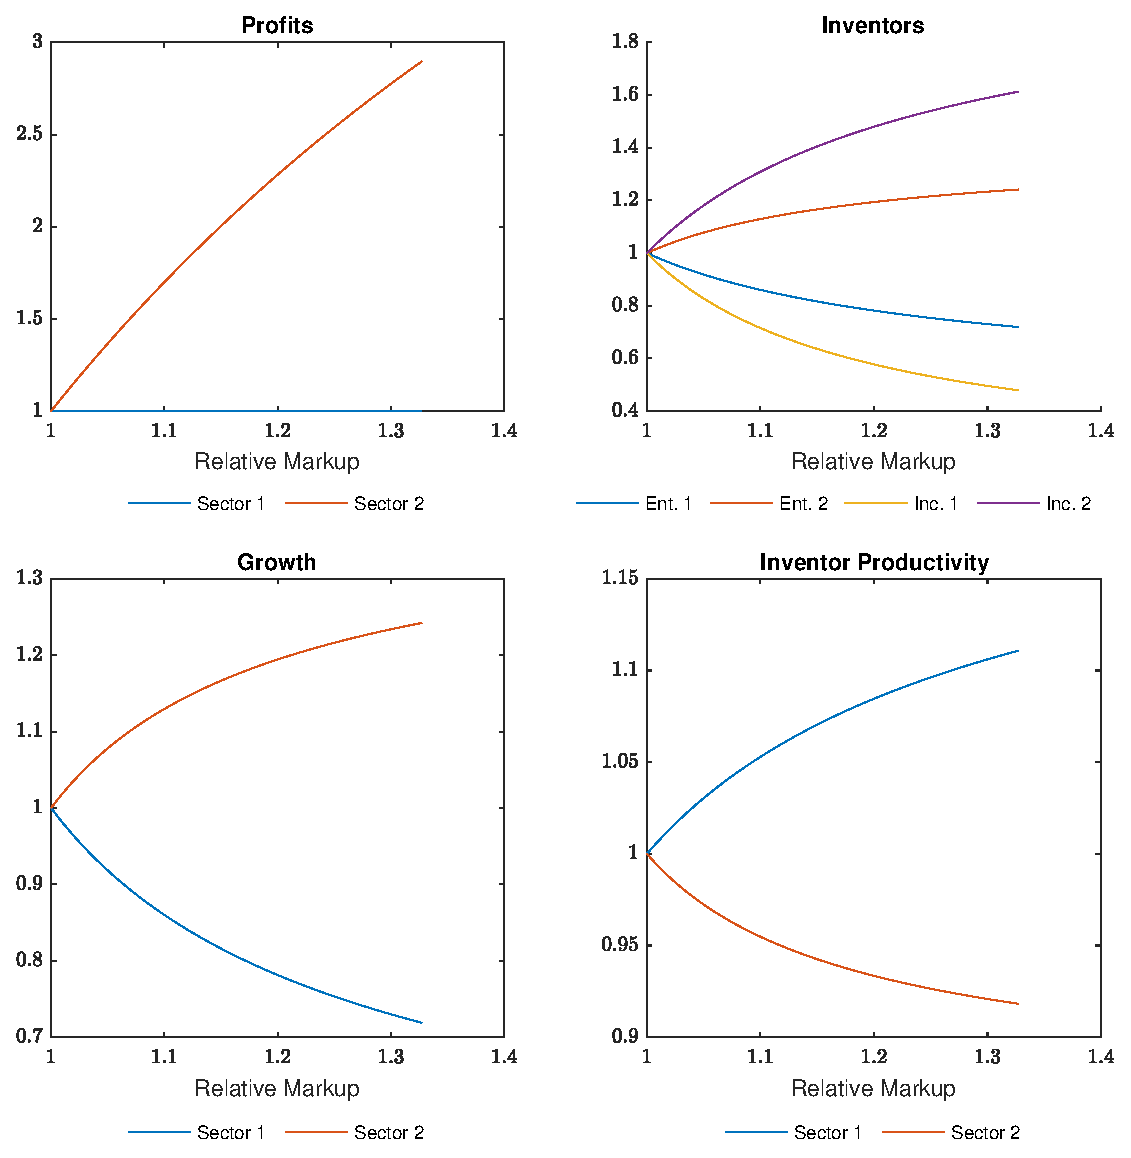
\includegraphics[width=0.65\textheight]{graphs/GE_sectors}
\end{figure}
\par\end{center}

\end{frame}
%

\end{document}
